\chapter{Моделирование работы искусственного сердечного клапана} \label{chapt3}

Как отмечалось ранее, искусственные сердечные клапаны являются одними из самых
сложных биопротезов, используемых в кардиохирургии. Они достаточно эффективно
позволяют бороться с заболеваниями и повреждениями естественных клапанов, но
при этом не являются достаточно долговечными и при их использовании могут
проявляться побочные явления. Например, механические клапаны обладают высокой
надежностью и долговечностью, но могут приводить к сильным деформациям потока,
формированию сгустков кровяных клеток и как следствие - к образованию тромбов.
Биологические клапаны лишены этого недостатка, однако они менее долговечны и их
изготовление достаточно сложная техническая задача, которая до сих пор
полностью не решена.

Данная глава посвящена результатам применения модели, описанной в главе \ref{chapt1},
для моделирования работы искусственного трехстворчатого клапана. Клапан расположен в
сосуде произвольной формы, закреплен фиброзным кольцом на его стенках, и приводится
в движение посредством перепада давления неоднородной несжимаемой жидкости в сосуде.
Эта модель применима, например, к аортальному клапану, который располагается на
границе левого желудочка и аорты, препятствуя обратному току крови из аорты в
левый желудочек на этапе диастолы.

Входными параметрами для данных расчетов являются:
\begin{itemize}
    \item Начальная форма клапана $\Gamma_4$ и сосуда $\Gamma_1$
    \item Жесткость клапана в каждой точке (коэффициенты $k_b$, $k_s$)
    \item Векторное поле скорости жидкости в начальный момент времени $\vec{u_0}$
    \item Распределение примеси в начальный момент времени
            (а соответственно, и концентрации $c_0$, вязкости $\mu_0$ и плотности $\rho_0$)
    \item Перепад давления $p_{in}$, $p_{out}$
\end{itemize}

В качестве результата моделирования мы получаем описание состояния системы
<<клапан-жидкость>> в каждый момент времени, т.е.:
\begin{itemize}
    \item Векторно поле скорости жидкости $\vec{u}$
    \item Скалярное поле давления жидкости $\vec{p}$
    \item Распределение примеси
    \item Текущая форма клапана
    \item Векторное поле напряжения деформации на поверхности клапана $F$
    \item Расход жидкости сквозь клапан
\end{itemize}

\section{Моделирование работы симметричного клапана} \label{sect3_1}

Одна из причин, по которой трехстворчатый сердечный клапан является крайне сложным
объектом для исследования, заключается в его сложной геометрии. Для каждого человека
она в той или иной степени уникальна, т.к. присутствуют отклонения от стандартной
формы. На первом этапе мы опустим эти сложности и будем рассматривать клапан идеальной
формы с тремя симметричными створками. Его схема изображена на рис. \ref{img:symmetric_valve}

\begin{figure}[H]
  \center
  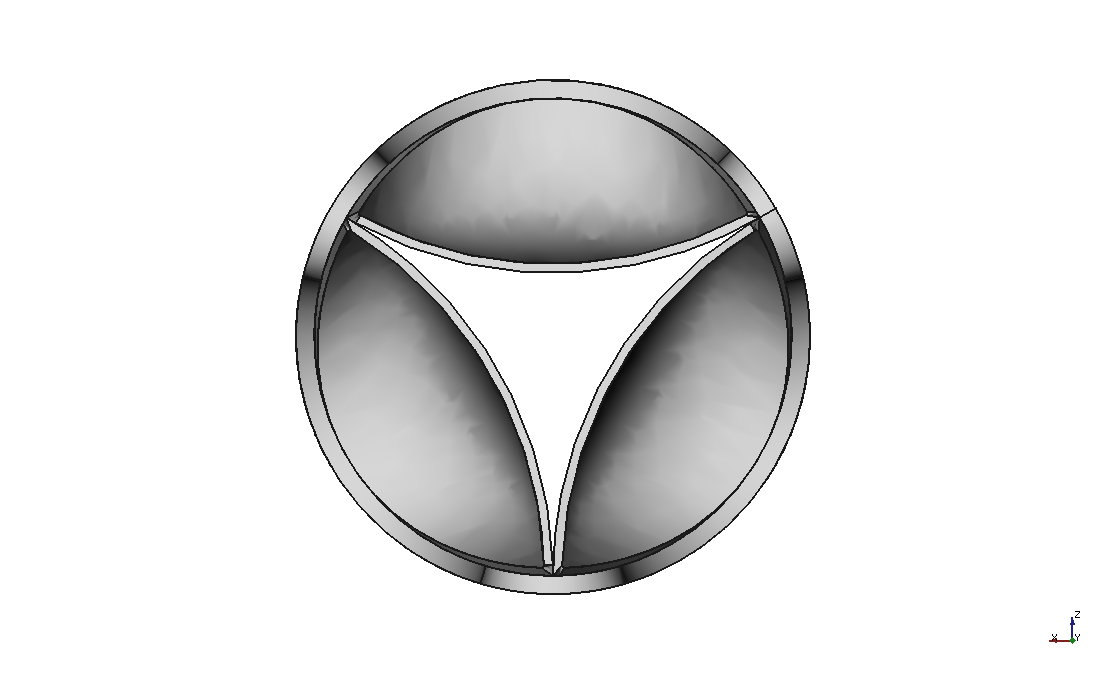
\includegraphics [scale=0.27] {SymmetricValveFront.png}
  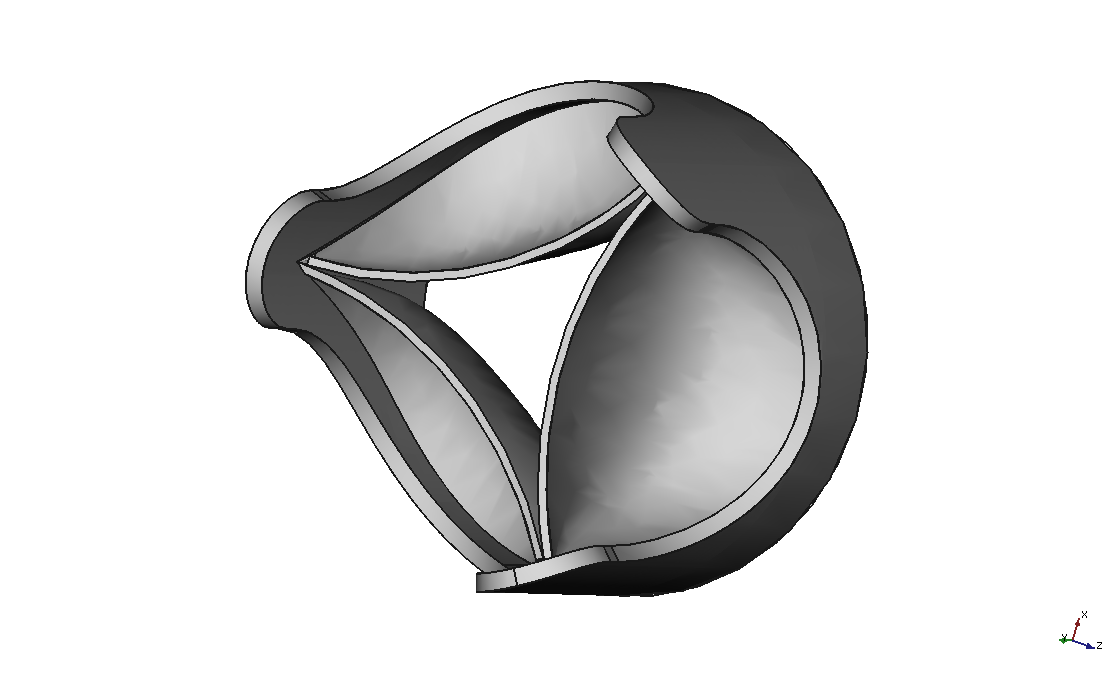
\includegraphics [scale=0.27] {SymmetricValveSide.png}
  \caption{Клапан идеальной формы с тремя симметричными створками}
  \label{img:symmetric_valve}
\end{figure}

Т.к. фиброзное кольцо в данном случае полностью совпадает с поверхностью сосуда,
в котором находится клапан, и стенки сосуда являются твердыми, мы можем его убрать,
переместив всю жесткость кольца на линию, по которой лепестки клапана соединяются
со стенками сосуда. Итоговая схема расчета изображена на рис. \ref{img:aorta_valve_scheme_flat}

\begin{figure}[H]
  \center
  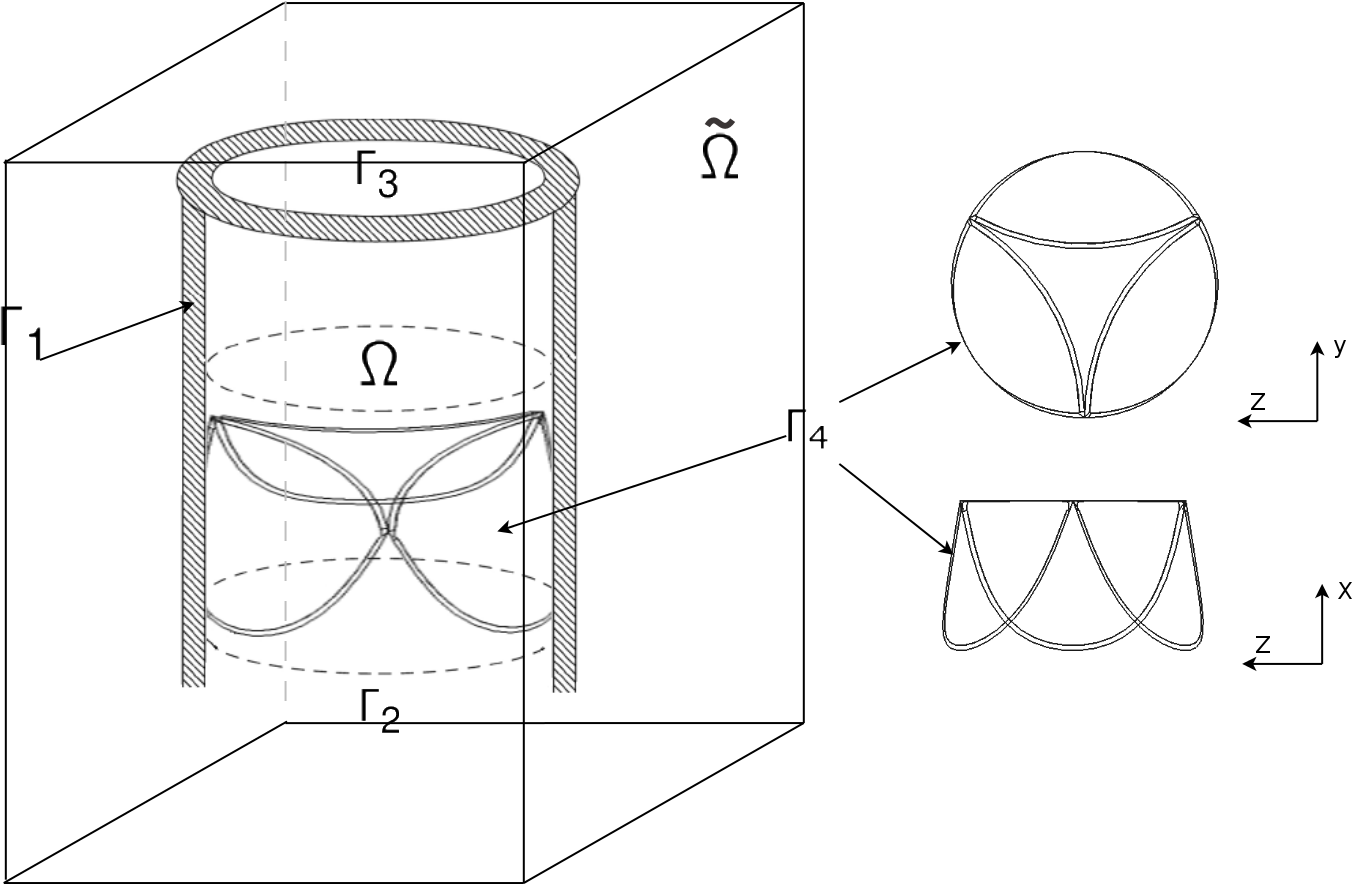
\includegraphics [scale=0.27] {aorta_valve_scheme_flat_computation.png}
  \caption{Схема расположения клапана в сосуде}
  \label{img:aorta_valve_scheme_flat}
\end{figure}

Все описанные ниже расчеты проводились в безразмерных переменных.  В качестве
сосуда, в котором расположен клапан, используется круговой цилиндр длинной $l=1$,
радиусом $r=0.11$. Для стенок сосуда используется <<простая>> формула расчета
напряжения (\ref{eq:simple_force}) с коэффициентом жесткости $k=1 \cdot 10^{3}$.
Область $\tilde{\Omega}$ имеет размеры $10 \times 0.5 \times 0.5$.

При проектировании искусственных сердечных клапанов одним из самых главных его свойств
является полнота закрытия створок в момент диастолы, т.к. это основная функция
створчатого аппарата. Ниже на рис. \ref{img:valve_delaunay_with_markers}
приведены результаты моделирования одного цикла работы клапана
при периодически меняющемся от $0$ до $6$ перепаде давления $p_{in} - p_{out}$,
параболической зависимостью от времени на каждом периоде.
Для створок клапана заданы коэффициенты сопротивления растяжению $k_s = 5 \cdot 10^{3}$ и скручиванию
$k_b = 2 \cdot 10^{3}$. Внутри сосуда течет вязкая однородная несжимаемая жидкость $\rho=1$, $\mu=1\cdot10^{-2}$.
Для расчета задавалась конечно-разностная сетка $\tilde{\Omega_h}$, соответствующая области течения,
и неструктурированная сетка $\tilde{\Gamma_h}$, соответствующая стенками сосуда и створкам клапана.
Расстояние между узлами $\tilde{\Omega_h}$ $h_x = h_y = h_z = 0.01$. Сетка $\tilde{\Gamma_h}$
была получена путем конвертирования CAD модели идеального клапана в сеточный формат с расстояниями
между узлами меньше соответствующих $h_x, h_y, h_z$ и количеством узлов $n=3021$.
Для рассчета был выбран шаг по времени $\triangle t = 0.01$.

\begin{figure}[H]
  \center

  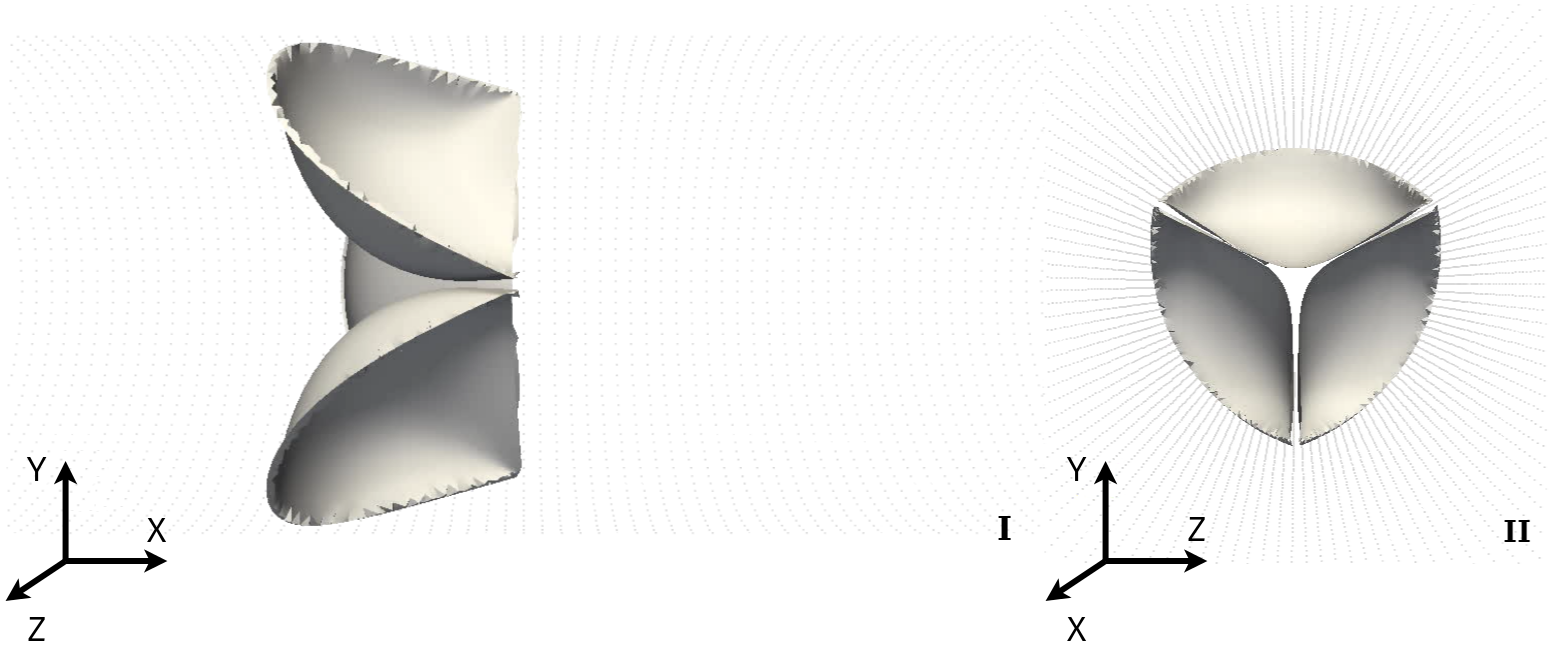
\includegraphics [scale=0.27] {valve_delaunay_with_markers1_axes.png}

  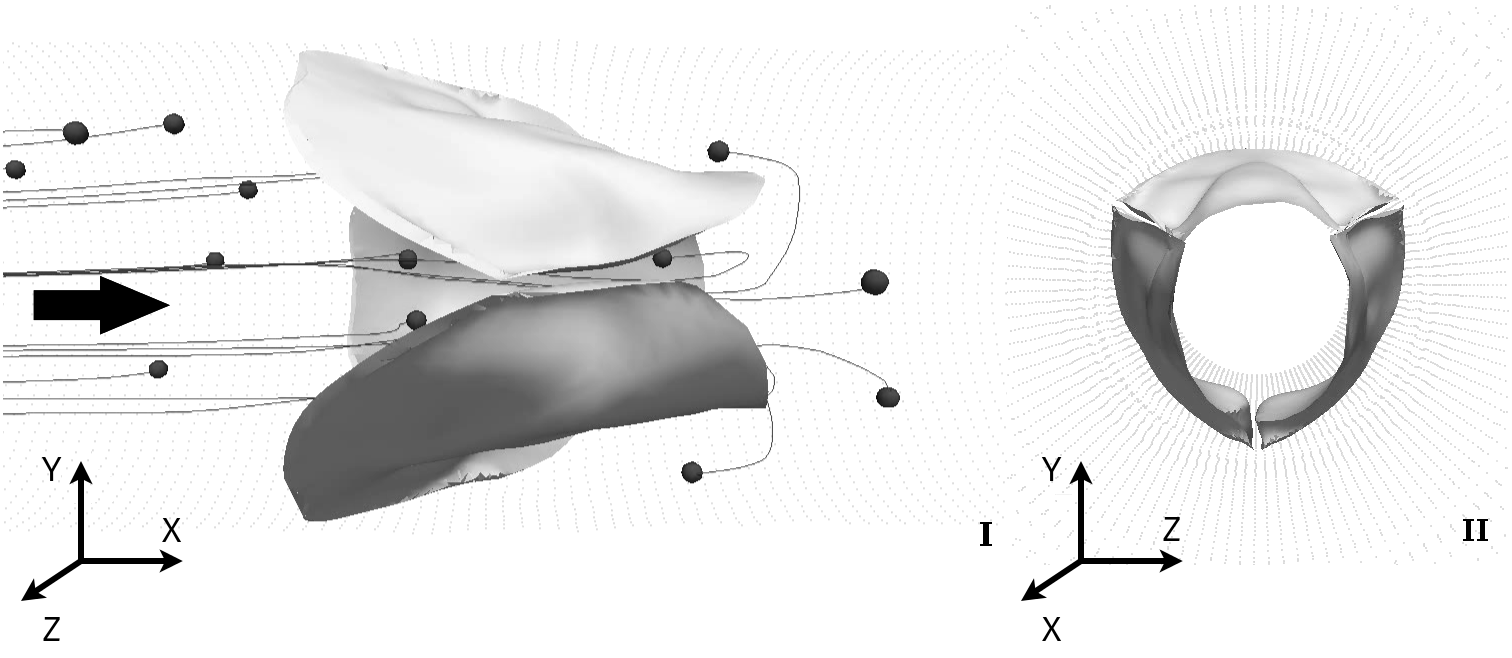
\includegraphics [scale=0.27] {valve_delaunay_with_markers2_axes.png}

  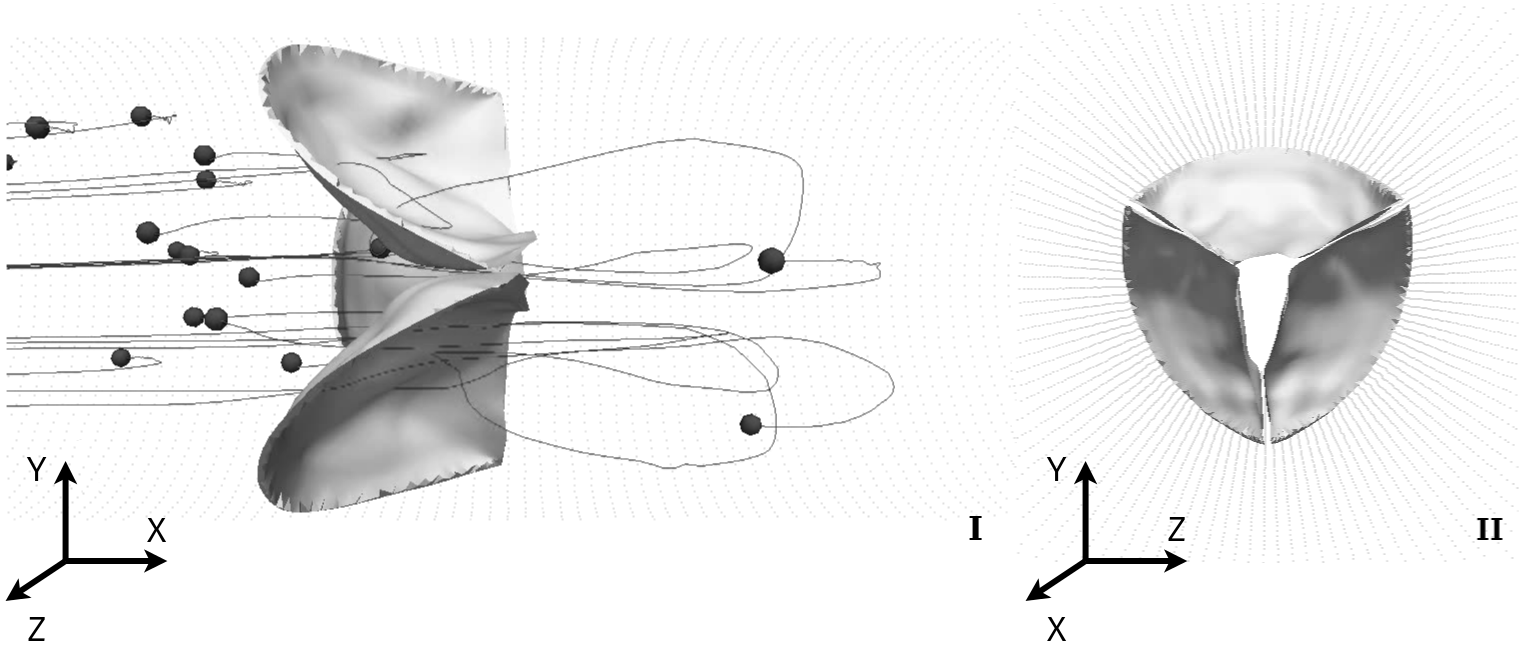
\includegraphics [scale=0.27] {valve_delaunay_with_markers3_axes.png}

  \caption{Динамика створок клапана и треки некоторых частиц. Направление тока
    указано стрелкой. Показан вид сбоку (I) и вид спереди (II) a) $t=0$, b)
    $t=0.7$, c) $t=1.5$}

  \label{img:valve_delaunay_with_markers}
\end{figure}

Этот расчет демонстрирует динамику формы створок клапана, а также треки частиц
жидкости, протекающей сквозь него. Створки клапана раскрываются при изменении
разности давлений, а затем возвращаются в исходное положение при выравнивании
давлений. В процессе движения створок возникают вихревые движения жидкости, при
закрытии часть жидкости успевает проникнуть назад через клапан до его закрытия
(так называемый, <<объем регургитации>>). В силу изначальной геометрии клапана
его закрытие происходит не полностью, т.к. перепад давления сильно отличается
от реалистичного, а также стенки сосуда являются абсолютно ровными, тогда как
в настоящих биологических системах на плотность закрытия клапана влияет наличие,
например, синусов Вальсальвы, которые деформируют течение.

Как было сказано ранее, во многих работах недостаточно акцентируется внимание
на влиянии течения жидкости на итоговое состояние системы. И одним из важных
аспектов нашей работы являются результаты моделирования работы трехстворчатого
клапана с учетом неоднородной структуры жидкости, протекающей сквозь него.

На рис. \ref{img:concentration_dynamics} показано изменение концентрации
форменных элементов при прохождении потока жидкости через клапан.
Большинство параметров для этого расчета аналогичны предыдущему,
за исключением того, что в сосуде течет неоднородная двухкомпонентная жидкость.
В начальный момент времени концентрация примеси в каждой точке равна
$c_0=0.45$, на входе задается постоянный приток примеси $c_s|_{\Gamma_2} = 0.45$.

\begin{figure}[H]
  \center

  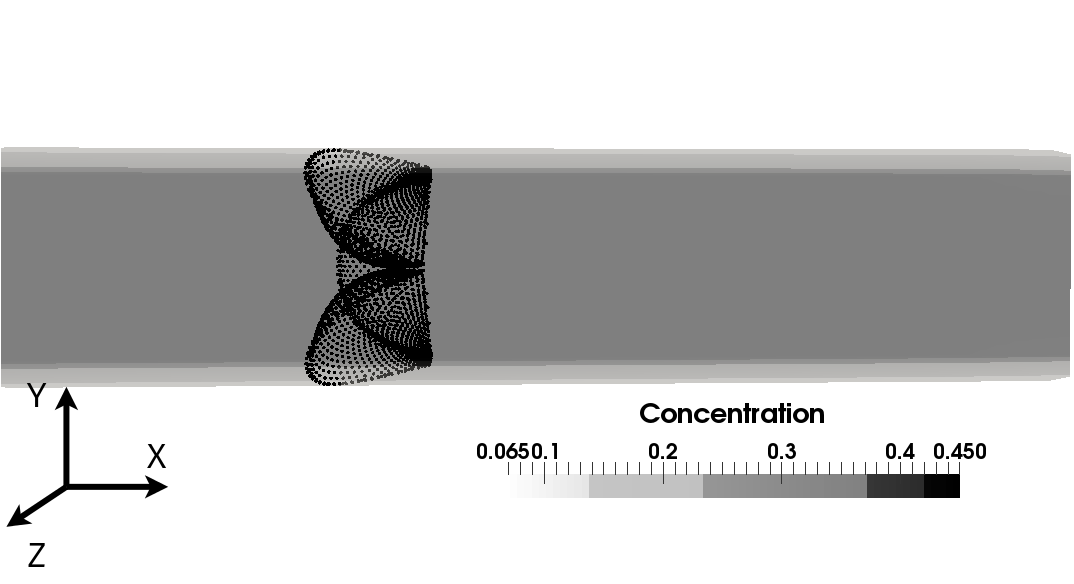
\includegraphics [scale=0.27] {concentration_1_axes.png}

  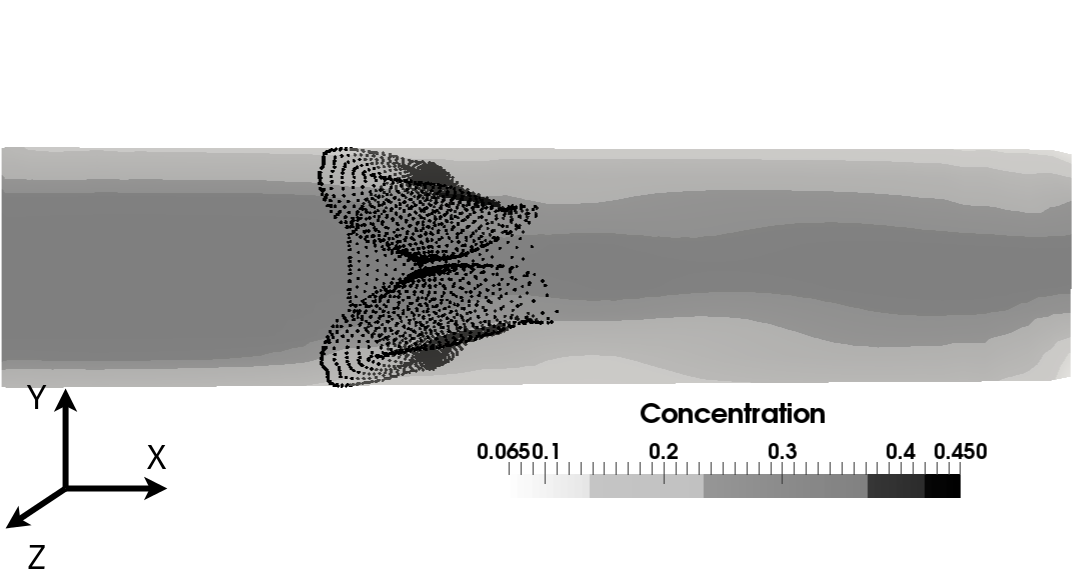
\includegraphics [scale=0.27] {concentration_2_axes.png}

  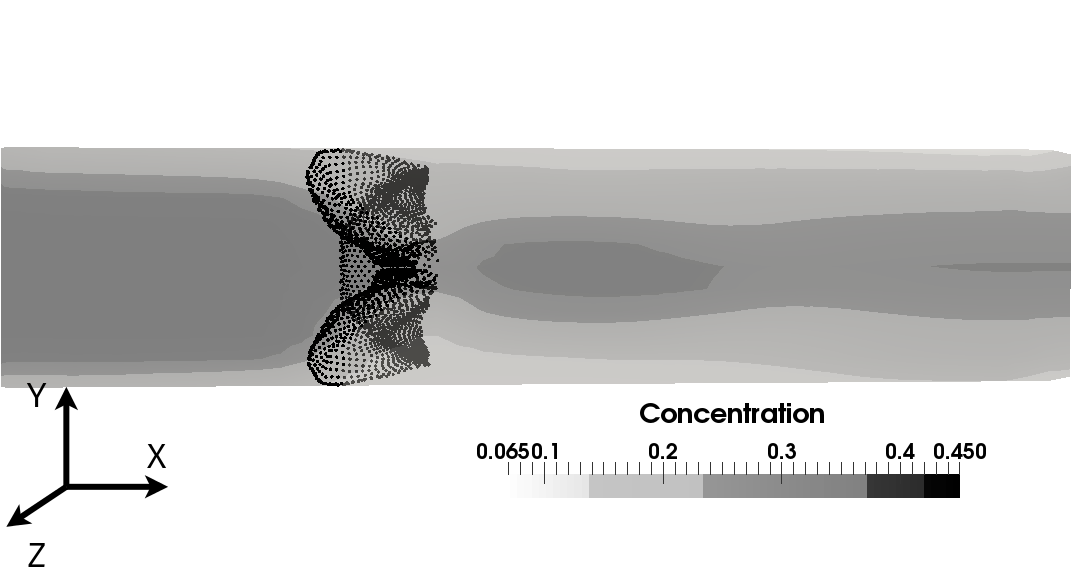
\includegraphics [scale=0.27] {concentration_3_axes.png}

  \caption{Движение створок клапана в сосуде с переменной вязкостью и плотностью.
    На входе задается постоянный приток примеси $c_s|_{\Gamma_2} = 0.45$,
    концентрация примеси в начальный момент времени $c_0=0.45$, $\rho_1=1,
    \rho_2=1.2, \mu_1=1 \cdot 10^{-2}, \mu_2=1.2 \cdot 10^{-2}$; a) $t=0$, b) $t=3$, c) $t=6$}

\label{img:concentration_dynamics}
\end{figure}

Финальное распределение показано после трех циклов работы клапана. Изначально
равномерное распределение форменных элементов со временем нарушается движением
створок клапана, приобретая пульсовый характер. Т.к. сам клапан не симметричен
по осям $Ox, Oy, Oz$, распределение примеси также не симметрично.

Но помимо неоднородной структуры жидкости крайне важным является итоговое
распределение напряжения деформации по поверхности створок клапана в разные
моменты времени, т.к. напряжение непосредственно влияет на его износ. Ниже
на рис. \ref{img:valve_stress_distribution} приведена динамика движения одной
из трех створок потоке неоднородной двухкомпонентной жидкости, а также визуализация
возникающего на ней напряжения.

\begin{figure}[H]
  \center

  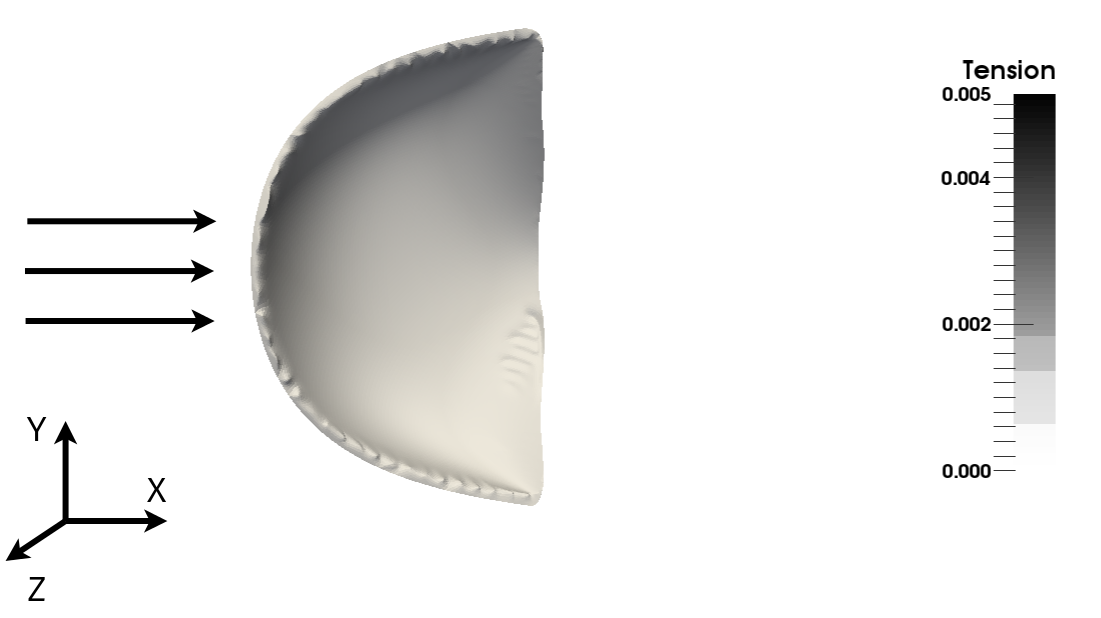
\includegraphics [scale=0.27] {ideal_valve_stress_1_better_axes.png}

  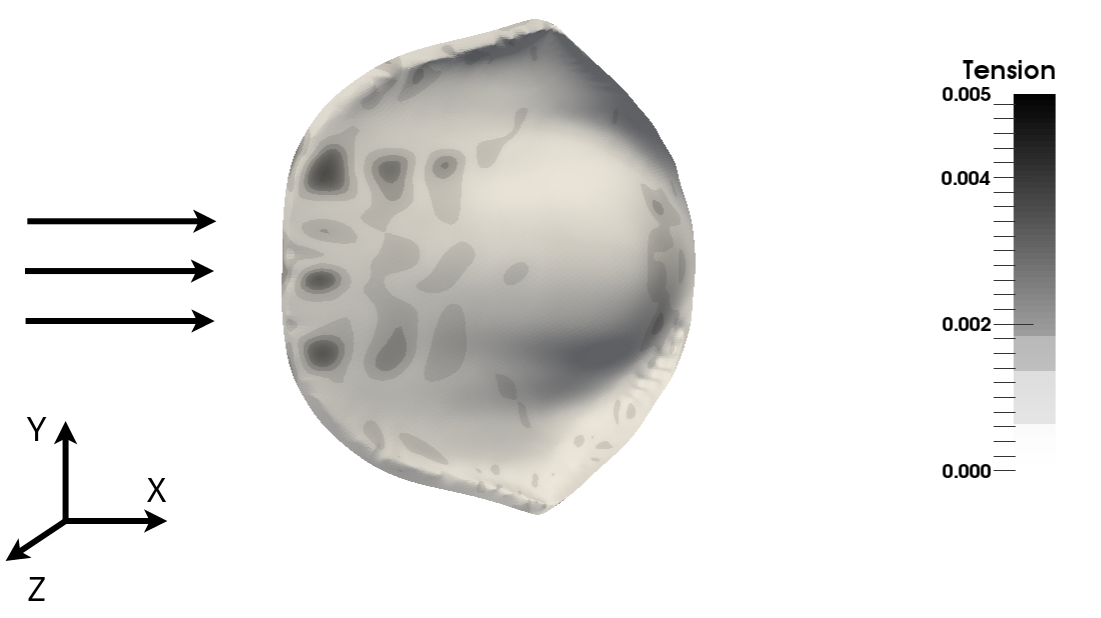
\includegraphics [scale=0.27] {ideal_valve_stress_2_better_axes.png}

  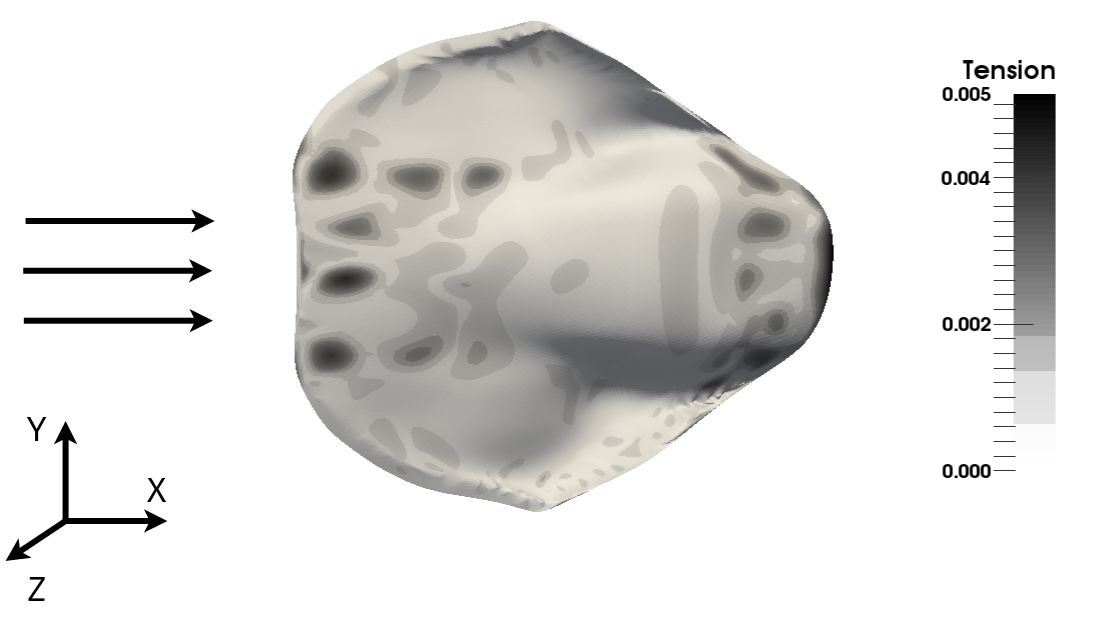
\includegraphics [scale=0.27] {ideal_valve_stress_3_better_axes.png}

  \caption{Распределение напряжение по поверхности створки в моменты времени $t=0, t=0.4, t=0.8$.
      Стрелками указано направление течения, под воздействием которого
    створка клапана деформируется.}

\label{img:valve_stress_distribution}
\end{figure}

В данном расчете при раскрытии створок больше поверхностного напряжения
возникает в двух областях - на конце створки, т.к. это самая гибкая его часть,
которая подвержена наибольшим деформациям скручивания, и в области крепления
створки к фиброзному кольцу, т.к. там возникает наибольшая деформация
растяжения в силу фиксированного расположения.

\section{Моделирование работы клапана <<Юнилайн>>} \label{sect3_2}

Следующим приближением для моделирования работы искусственного сердечного
клапана в данной работе являлось использование более реалистичной геометрии
створок. Для этого был использован искусственный клапан <<Юнилайн>>,
разработанный в ФГБУ НИИ КПССЗ СО РАМН, г. Кемерово (см. рис. \ref{img:uniline_real}
и \cite{klyshnikov2013comparison}). Клапан был отсканирован и преобразован в CAD
модель (рис. \ref{img:uniline_cad}).

\begin{figure}[H]
  \center
  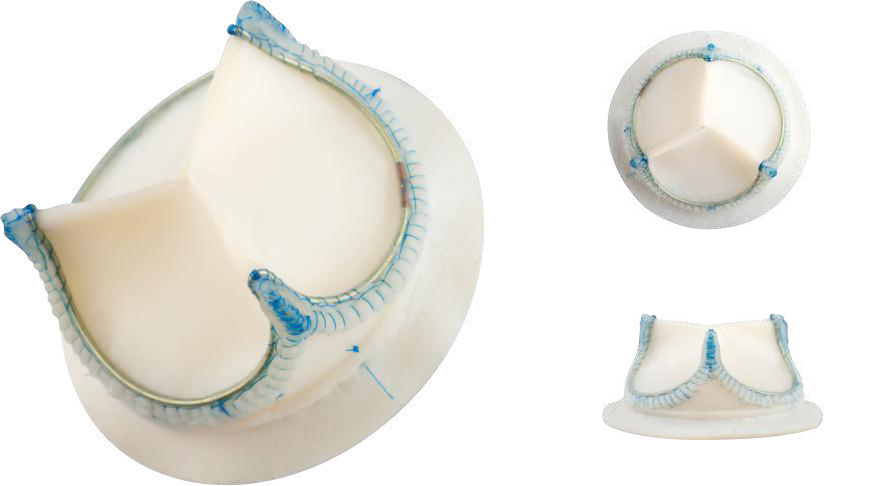
\includegraphics [scale=0.6] {uniline_real_no_alpha.png}
  \caption{Искусственный клапан <<Юнилайн>>}
\label{img:uniline_real}
\end{figure}

\begin{figure}[H]
  \center
  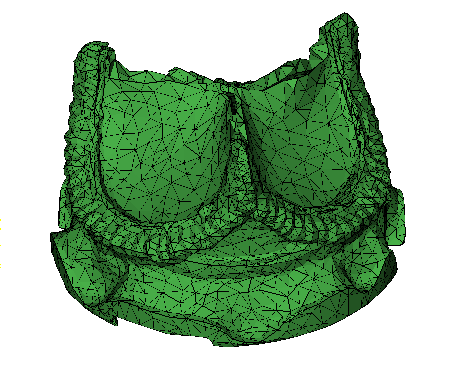
\includegraphics [scale=0.7] {real_valve_3_1.png}
  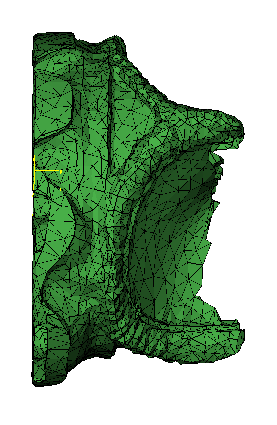
\includegraphics [scale=0.6] {real_valve2_1.png}
  \caption{CAD модель клапана <<Юнилайн>>}
\label{img:uniline_cad}
\end{figure}

Клапан состоит из трех гибких несимметричных створок, твердого фиброзного
кольца, который закрепляется на сосуде, а также трех стоек для крепления
створок клапана. Отличительной особенностью данного клапана является то, что
при закрытии створки перекрывают друг друга.

Для этого клапана мы провели ряд расчетов, схожих с описанными выше для клапана
симметричной формы. Использовались следующие коэффициенты для расчета напряжения
клапана - $k_s = 10 \cdot 10^3$, $k_b = 2 \cdot 10^3$. Для напряжения фиброзного
кольца и стоек использовалась <<простая>> формула расчета
напряжения (\ref{eq:simple_force}) с коэффициентом жесткости $k=2 \cdot 10^{3}$.
Перепад давления $p_{in} - p_{out}$ периодически изменялся от $-2$ до $7$.
Внутри сосуда течет вязкая однородная несжимаемая жидкость $\rho=1$, $\mu=1\cdot10^{-2}$.

\begin{figure}[H]
  \center

  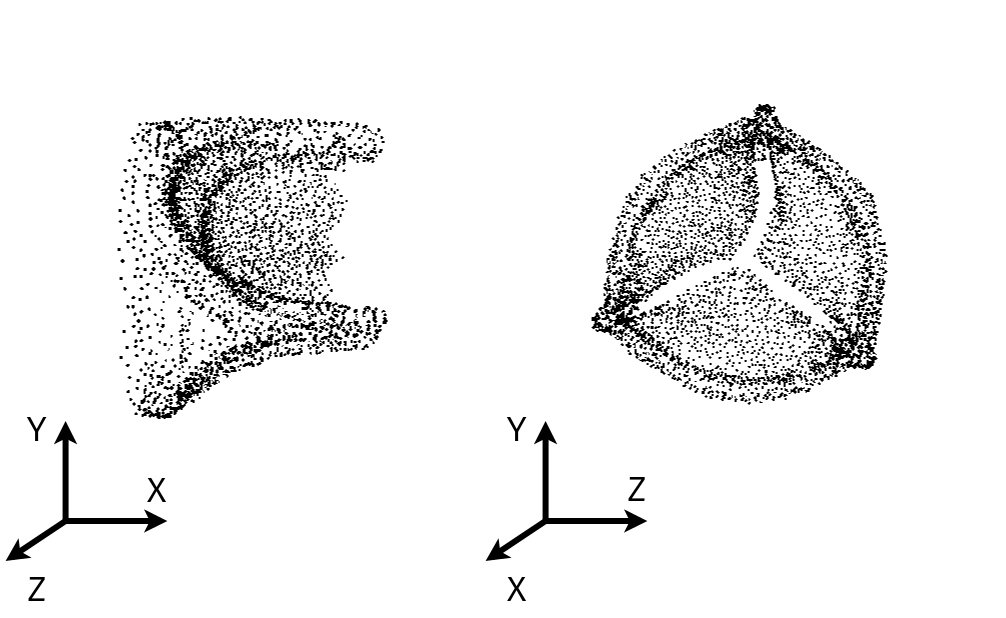
\includegraphics [scale=0.27] {uniline_dynamics_11_axes.png}

  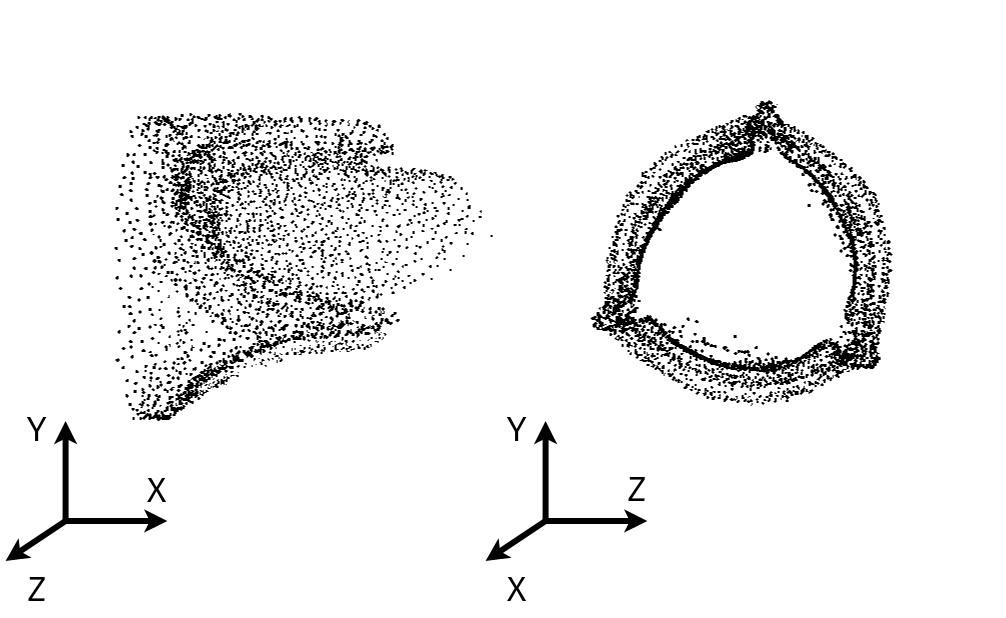
\includegraphics [scale=0.27] {uniline_dynamics_22_axes.png}

  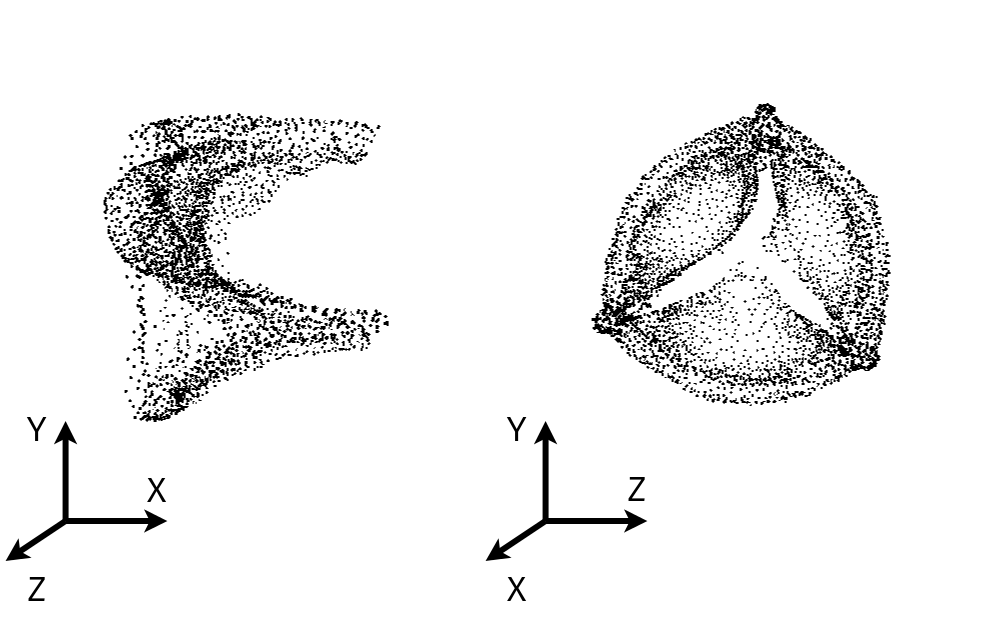
\includegraphics [scale=0.27] {uniline_dynamics_33_axes.png}

  \caption{Работа клапана в моменты времени $t=0, t=0.5, t=1.8$. Точками обозначена
    поверхность фиброзного кольца и створки клапана. Коэффициенты жесткости
    $k_s = 10 \cdot 10^3$, $k_b = 2 \cdot 10^3$.}

\label{img:uniline_dynamics}
\end{figure}

На рис. \ref{img:uniline_dynamics} представлена динамика исследуемого клапана при
данных условиях. При повышении давления на входе створки клапана раскрываются, почти
полностью открывая путь для потока жидкости. Затем при повышении давления $p_{out}$
створки схлопываются, преграждая путь для обратному потоку жидкости.

На динамику работы искусственного сердечного клапана существенное влияние оказывает
жесткость его компонент. Покажем это на примере рис. \ref{img:uniline_dynamics_hard},
где $k_b$ в момент систолы линейно увеличивается от $2 \cdot 10^3$ до $10 \cdot 10^3$.
Т.к. в используемой реализации метода погруженной границы есть проблемы со сходимостью
по времени, для этого расчета был уменьшен шаг по времени $\triangle t = 1 \cdot 10^{-3}$
Как видно из полученных результатов, закрытие клапана происходит быстрее и с меньшей
итоговой деформацией, т.е. начальное и конечное положения почти идентичны.

\begin{figure}[H]
  \center

  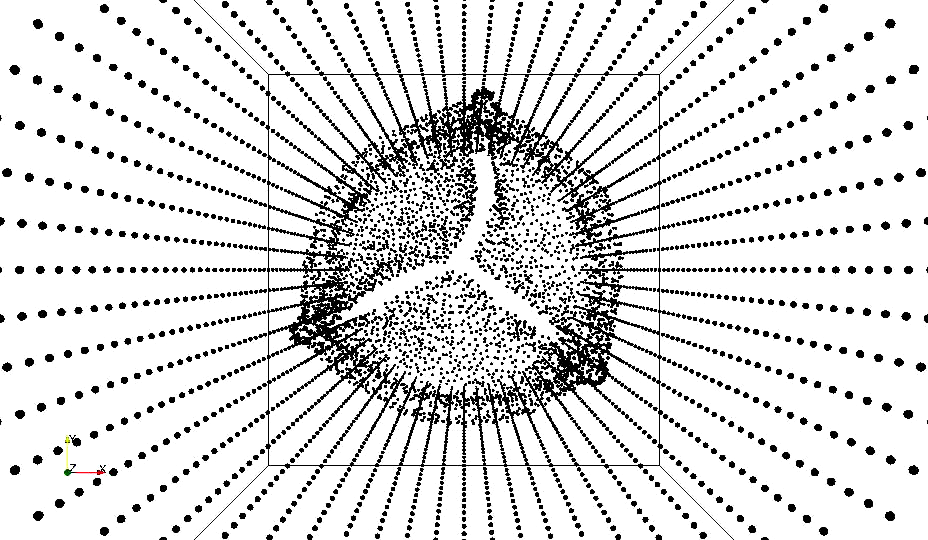
\includegraphics [scale=0.27] {uniline_dynamics_hard_1.png}

  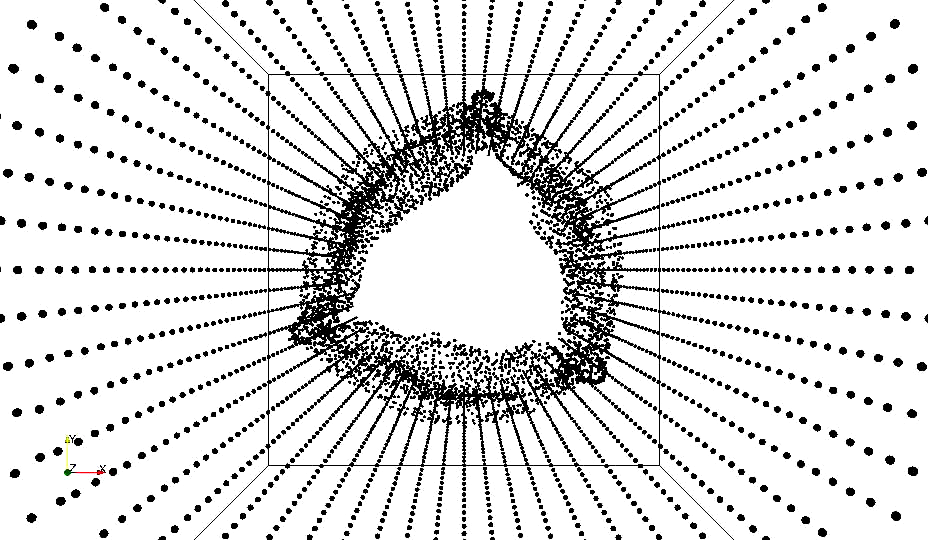
\includegraphics [scale=0.27] {uniline_dynamics_hard_2.png}

  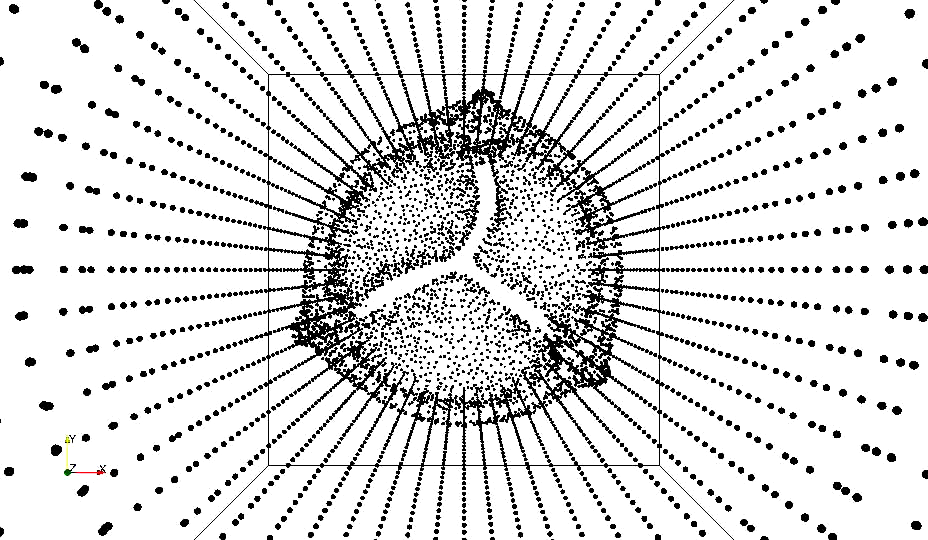
\includegraphics [scale=0.27] {uniline_dynamics_hard_3.png}

  \caption{Работа клапана в моменты времени $t=0, t=0.5, t=1.8$ вид с переди.
      Точками обозначена поверхность фиброзного кольца и створки клапана.
      Коэффициенты жесткости $k_s = 10 \cdot 10^3$, $k_b$ от $2 \cdot 10^3$ до $10 \cdot 10^3$.}

\label{img:uniline_dynamics_hard}
\end{figure}

Помимо этого существует большое количество других факторов, влияющих на работу искусственного
сердечного клапана, например, геометрия сосуда, в котором он установлен. На рис. \ref{img:uniline_in_cone}
показа динамика клапана <<Юнилайн>>, закрепленного на выходе из сосуда в прямоугольный канал
большего объема с твердыми стенками (см. рис. \ref{img:valve_out_of_aorta}).
На этих стенках задано условие прилипания, через всю противоположную границу $\Gamma_3$
происходит свободное вытекание жидкости.

\begin{figure}[H]
  \center
  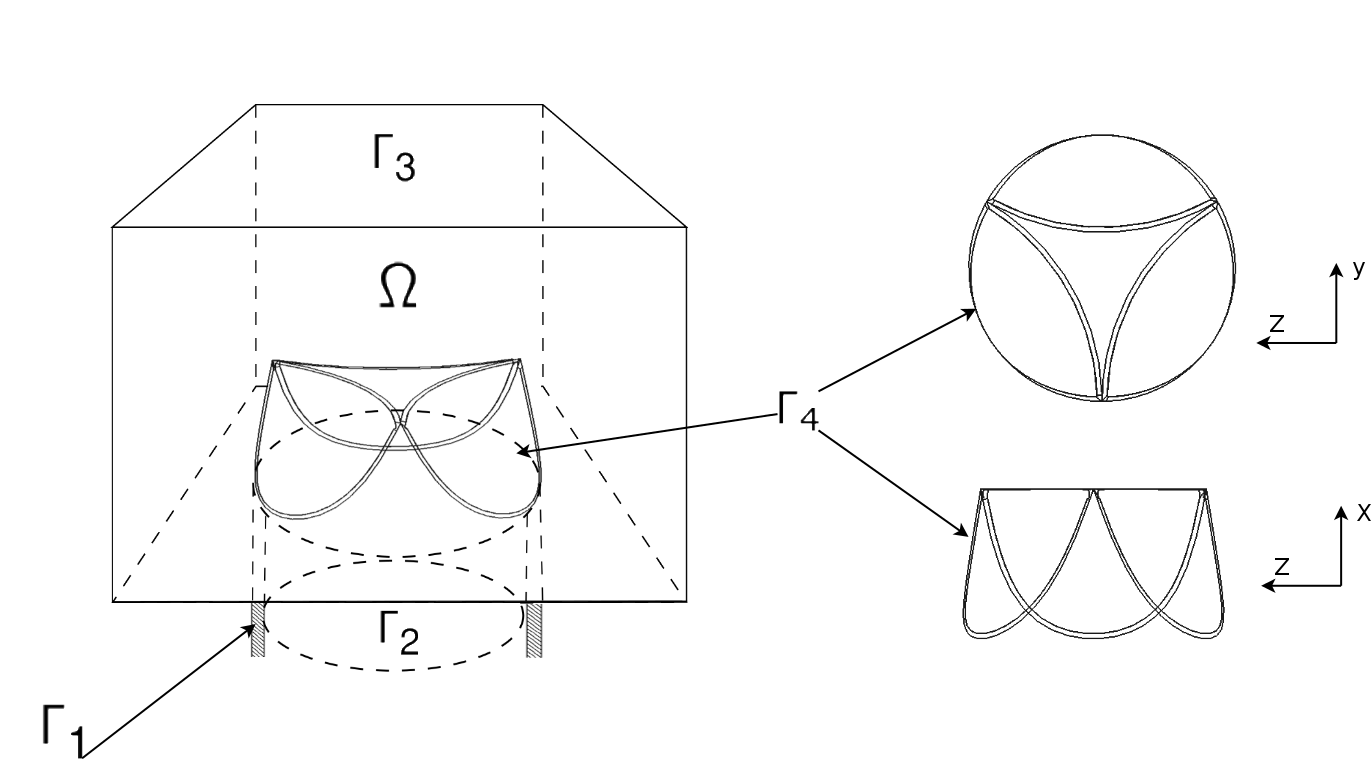
\includegraphics [scale=0.27] {valve_out_of_aorta.png}
  \caption{Схема расположения клапана на выходе из сосуда}
  \label{img:valve_out_of_aorta}
\end{figure}

\begin{figure}[H]
  \center

  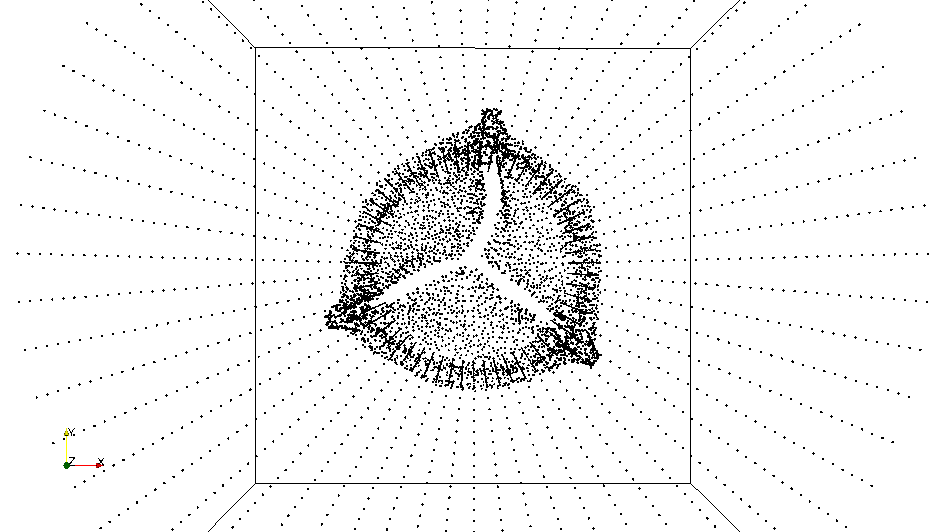
\includegraphics [scale=0.25] {different_valve_front_1.png}
  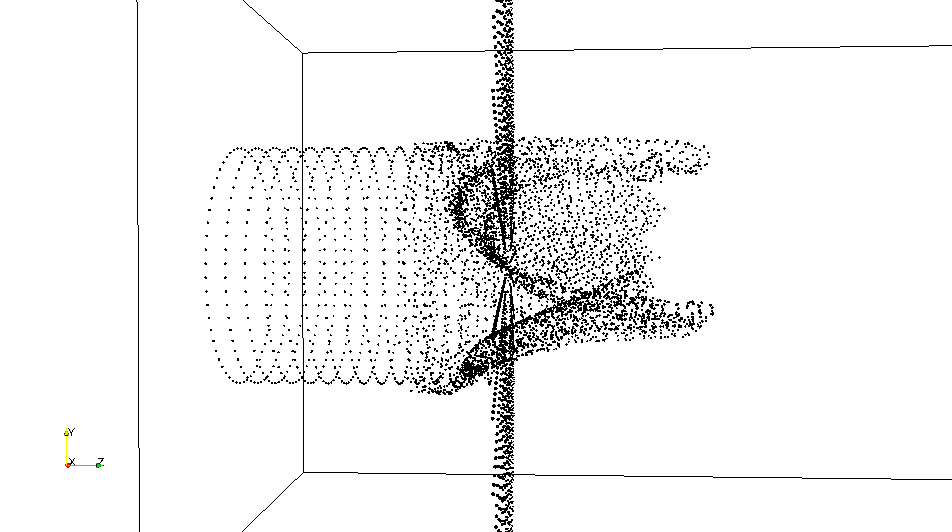
\includegraphics [scale=0.25] {different_valve_side_1.png}

  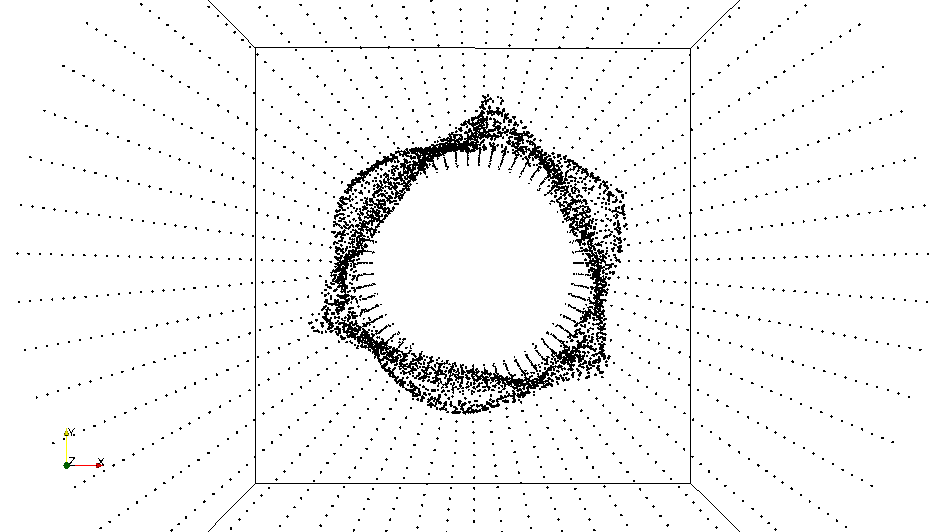
\includegraphics [scale=0.25] {different_valve_front_2.png}
  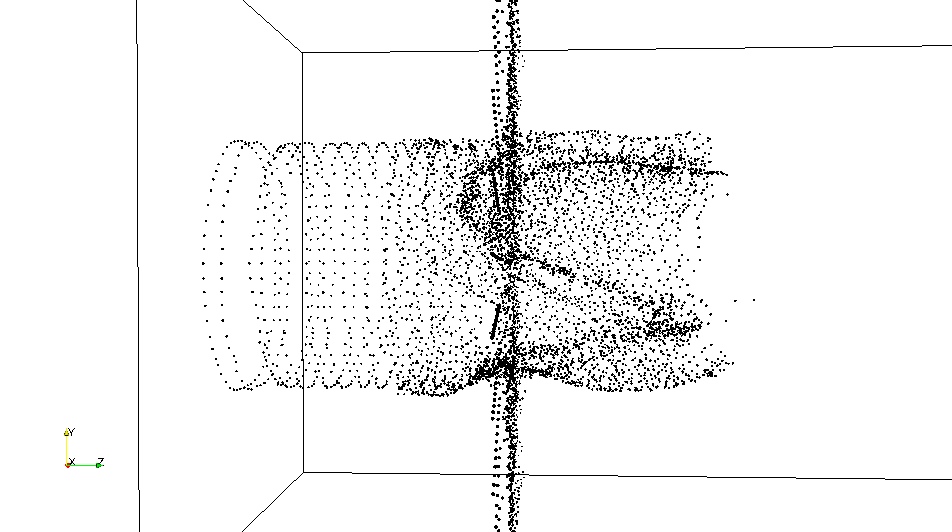
\includegraphics [scale=0.25] {different_valve_side_2.png}

  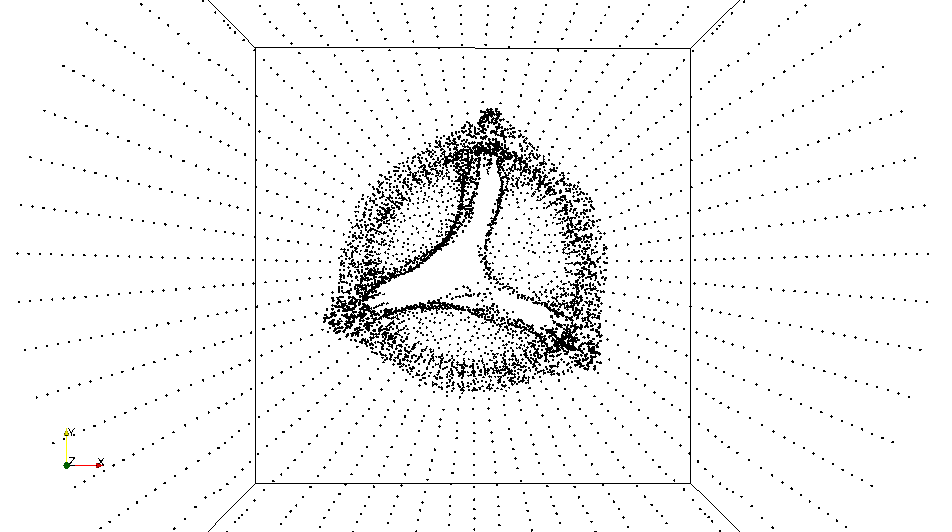
\includegraphics [scale=0.25] {different_valve_front_3.png}
  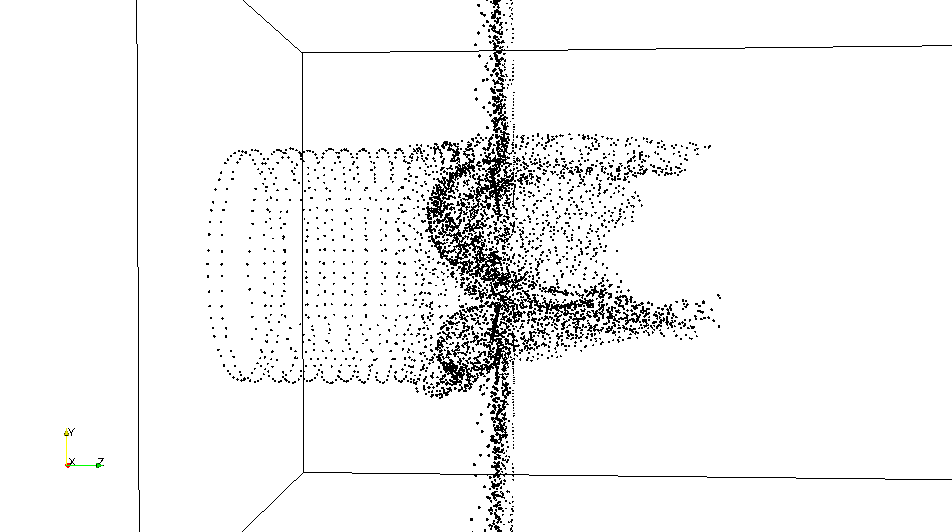
\includegraphics [scale=0.25] {different_valve_side_3.png}

  \caption{Динамика клапана <<Юнилайн>>, установленного на выходе из сосуда}

  \label{img:uniline_in_cone}
\end{figure}

Данное расположение клапана и форма сосуда, в котором он установлен, приводит к
другому виду потока жидкости через клапан. Это проявляется в том, что створчатый
аппарат раскрывается сильнее при тех же коэффициентах жесткости, что и для
предыдущих расчетов.

Другим важным фактором, значительно влияющим на работку искусственного клапана
является наличие примеси в жидкости и ее характеристики. Покажем это на примере
следующих расчетов, в который динамика клапана моделировалась при течении внутри
неоднородной жидкости. Параметры расчета эквивалентны рис. \ref{img:uniline_dynamics},
за исключением наличия примеси в начальный момент времени с концентрацией
$c(\bar{x}, 0) = 0.45$, плотностью и вязкостью $\rho=1.2, \mu=1.2 \cdot 10^{-2}$ и
условием поступления примеси через границу $\Gamma_2$, $c(\bar{x}, t)|_{\Gamma_2} = 0.45$.
Полученные результаты сравнивались работой клапана без примеси. Для этого были
выбраны три характерные точки на поверхности клапана (см. рис. \ref{img:valve_points}):

\begin{figure}[H]
  \center
  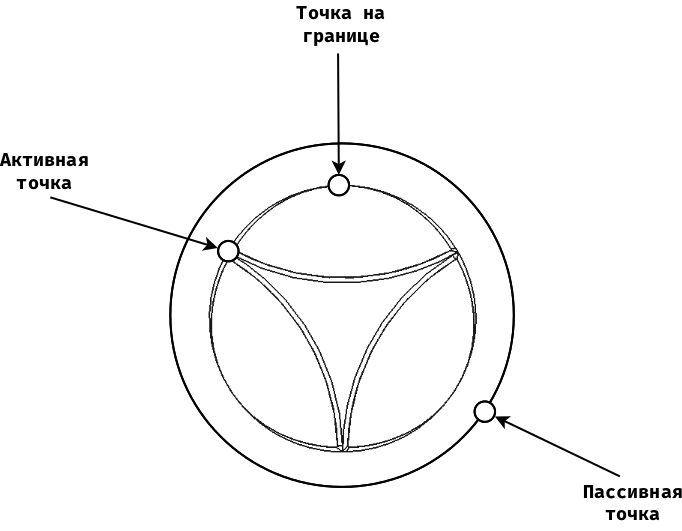
\includegraphics [scale=0.37] {valve_points.png}
  \caption{Схема расположения точек для измерения напряжения на поверхности клапана}
  \label{img:valve_points}
\end{figure}

\begin{itemize}
    \item <<Активная>> точка, которая расположена на стыке двух створок, где
    судя по экспериментальным данным, должно быть наибольшее напряжение
    при закрытии клапана
    \item <<Граничная>> точка, расположенная на стыке створки клапана и
    фиброзного кольца
    \item <<Пассивная>> точка, лежащая на фиброзном кольце
\end{itemize}

В этих точках измерялось результирующее напряжение На рис. \ref{img:forces_admixture_comparison} показано сравнение напряжения в этих точках для случая
с примесью и без нее в виде графика зависимости напряжения от времени.
На этих графиках можно отметить, что наличие примеси снижает абсолютную величину
напряжения и его изменение во времени происходит с некоторым смещением относительно графика без примеси.

\begin{figure}[H]
  \center

  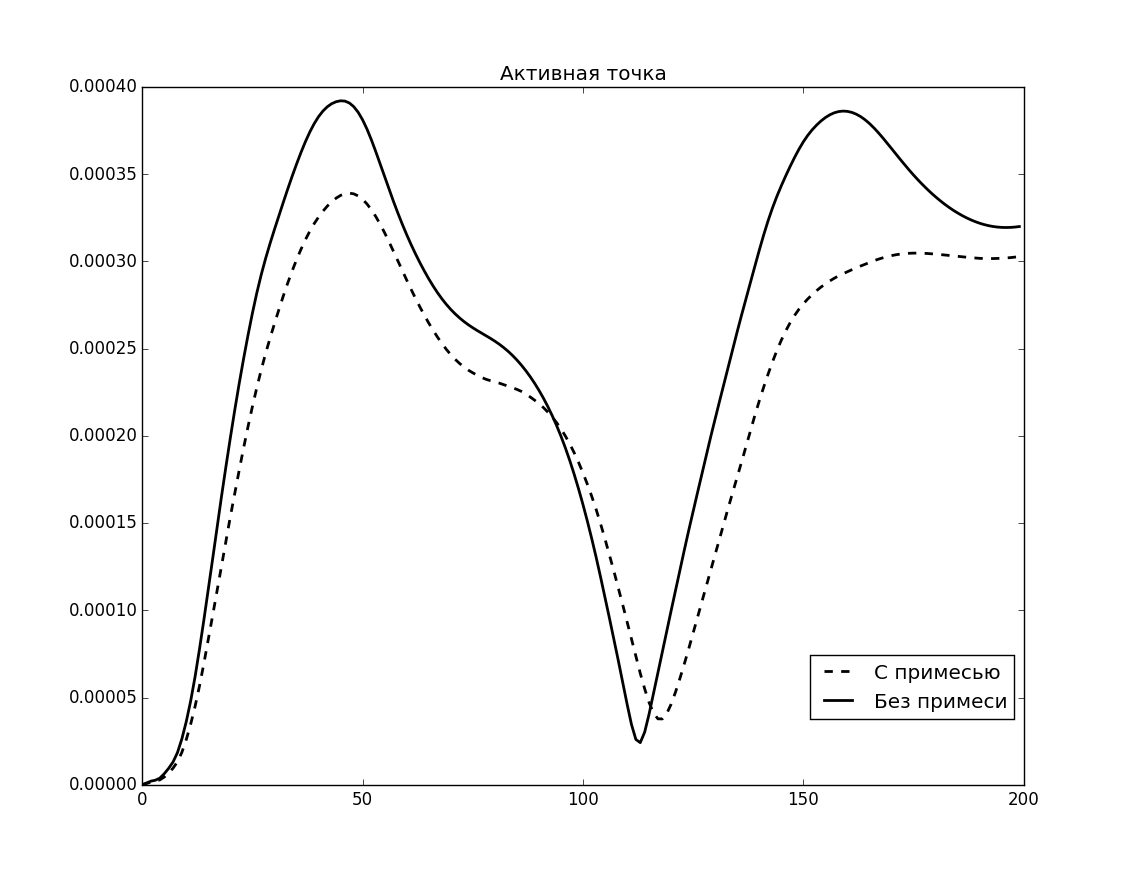
\includegraphics [scale=0.27] {forces_active_point.png}

  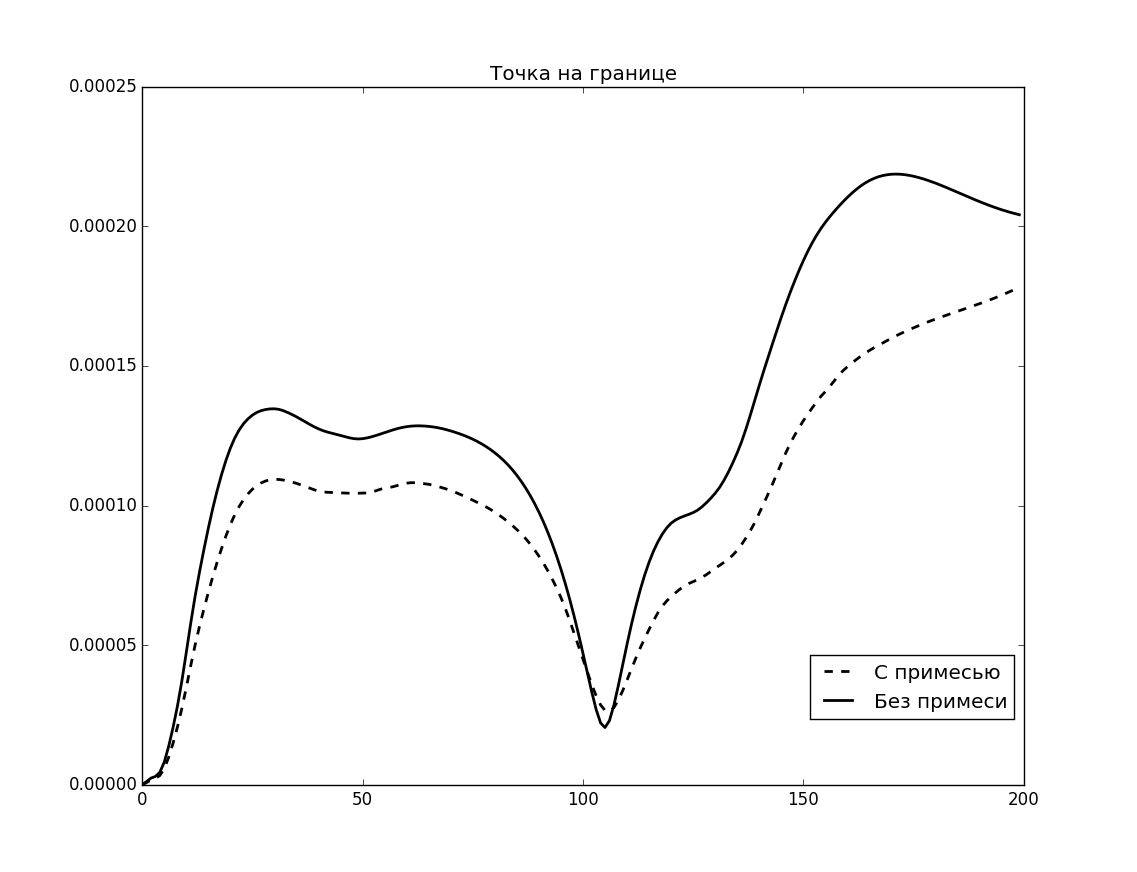
\includegraphics [scale=0.27] {forces_boundary_point.png}

  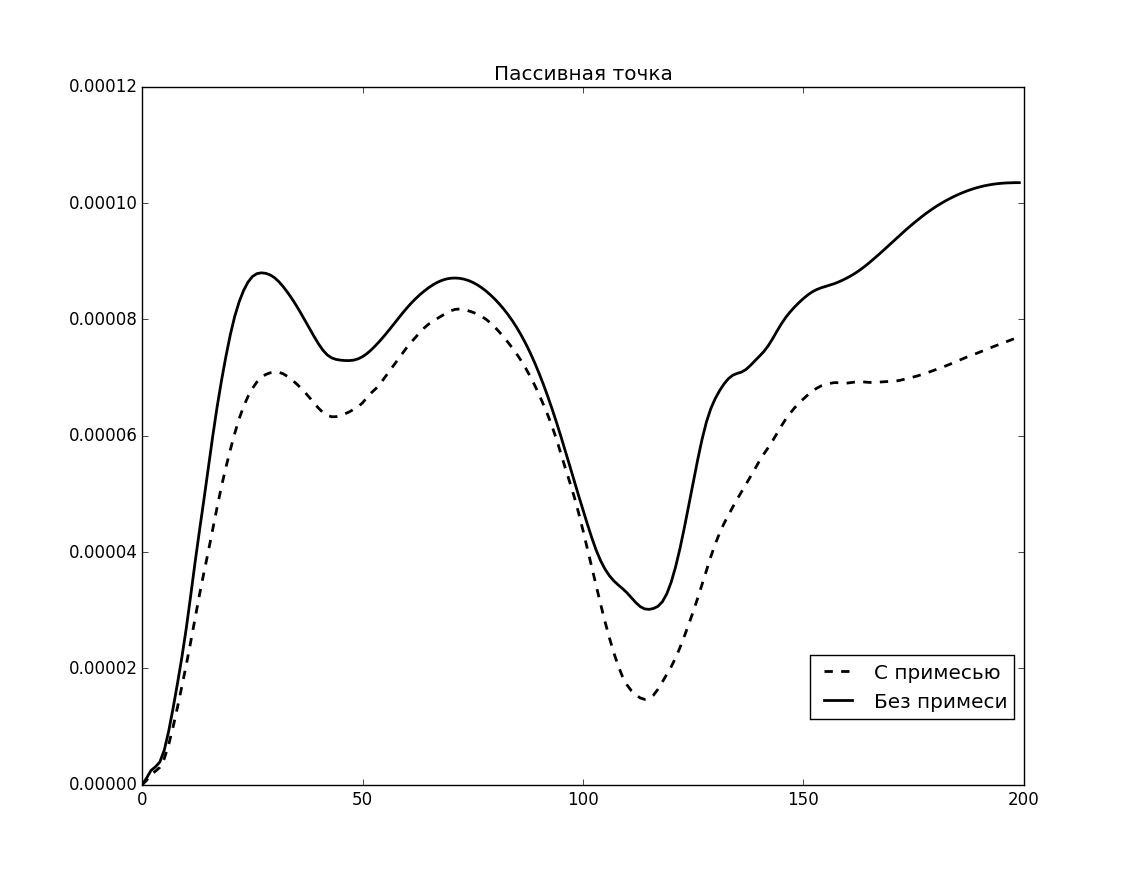
\includegraphics [scale=0.27] {forces_passive_point.png}

  \caption{Зависимость напряжения от времени для трех точек на фиброзном кольце
    для случаев без примеси (непрерывная линия) и с примесью (штриховая линия).
    На первом графике (a) изображена зависимость для "Активной точки", на
    втором (b) - для "Точки на границе", на третьем (c) - для "Пассивной
    точки"}

\label{img:forces_admixture_comparison}
\end{figure}

Однако на рис. \ref{img:forces_admixture_comparison} приведен только самый простой случай
влияния примеси на динамику жидкости, когда ее распределение изначально равномерно.
Более сложные виды распределения могут привести соответственно к иным картинам работы
клапана. Рассмотрим, например, результат работы клапана <<Юнилайн>> при попадании
в него сгустка примеси сферической формы (см. рис. \ref{img:thrombus_in_valve}).
Видно, что сгусток обладает достаточно вязкостью ($\mu_1 = 0.12$), и <<застревает>>
в клапане, выходя из него полностью только на втором цикле сокращений.

\begin{figure}[H]
  \center

  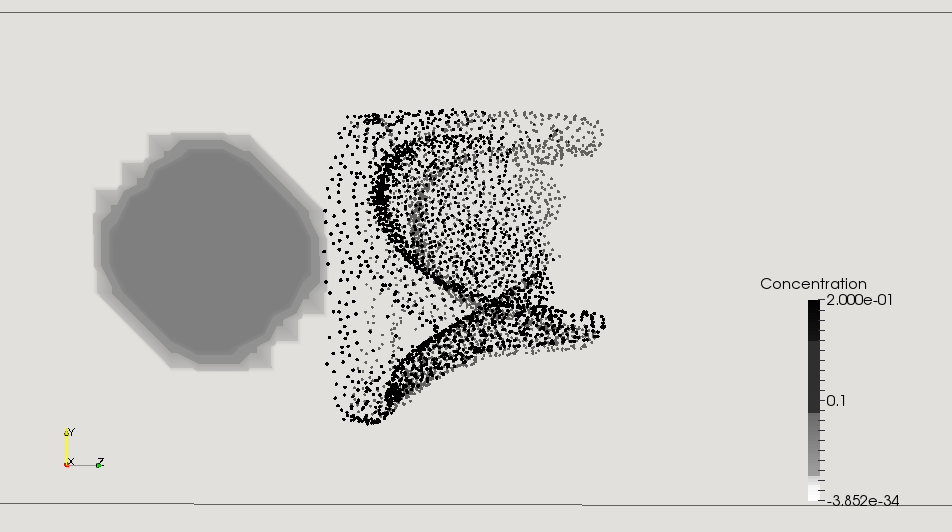
\includegraphics [scale=0.27] {thrombus_in_valve_1.png}

  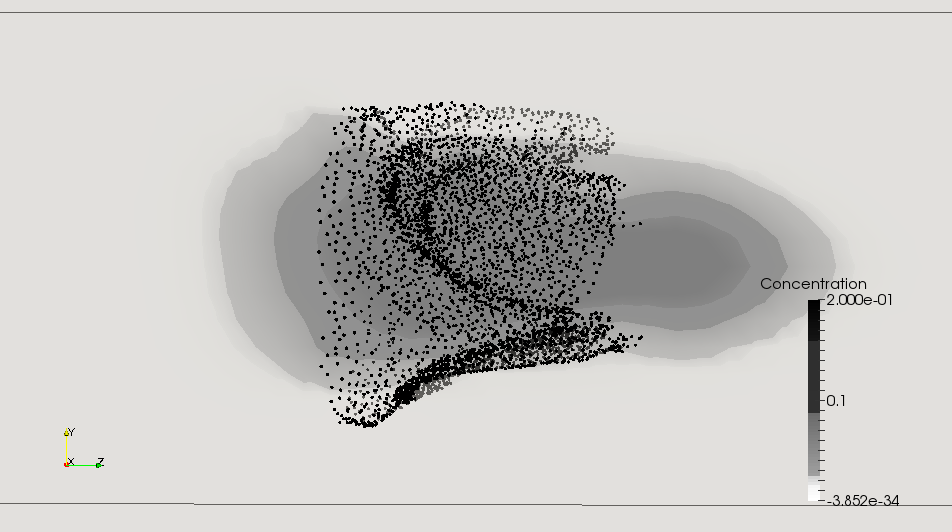
\includegraphics [scale=0.27] {thrombus_in_valve_2.png}

  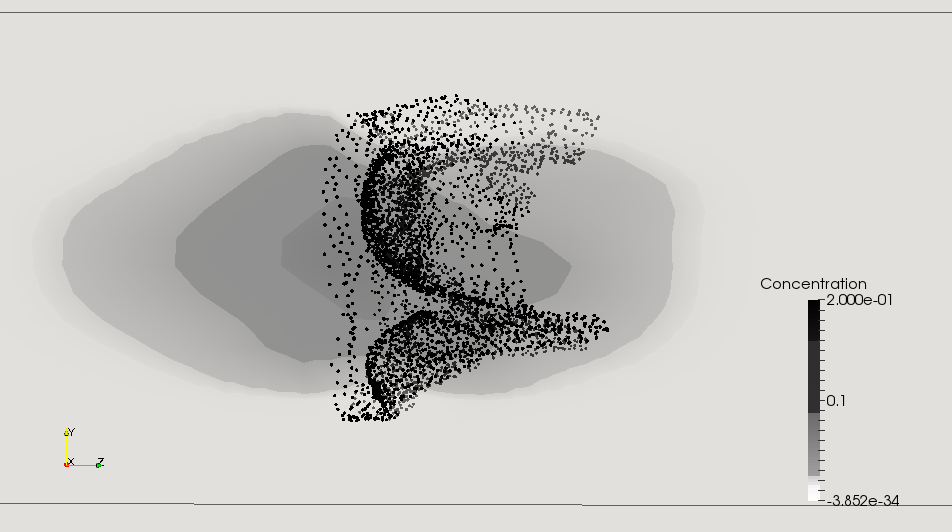
\includegraphics [scale=0.27] {thrombus_in_valve_3.png}

  \caption{Динамика работы клапана <<Юнилайн>> при попадании в него
           сгустка примеси. Приведен срез по центру сосуда с
           изображением концентрации примеси.}

\label{img:thrombus_in_valve}
\end{figure}

Для того, чтобы сравнить напряжение на поверхности клапана в случае однородной
жидкости и в случае попадания сгустка примеси, рассмотрим центральную точку
одной из его створок и измерим напряжение в ней для двух циклов работы клапана.
На рис. \ref{img:forces_thrombus_comparison} показано сравнение полученных графиков
изменения напряжения в зависимости от времени. Интересно, что если без сгустка примеси
пики напряжения соответствуют фазам работы створчатого аппарата и мы видим на графиках
подъемы и следующие за ним спады, то для случая с наличием примеси, картина немного другая.
Наличие сгустка в створчатом аппарате приводит к тому, что напряжение почти не спадает
между фазами работы клапана, что приводит к его постоянному росту. Очевидно, что это
в итоге приводит к серьезному нарушению работы клапана.

\begin{figure}[H]
  \center
  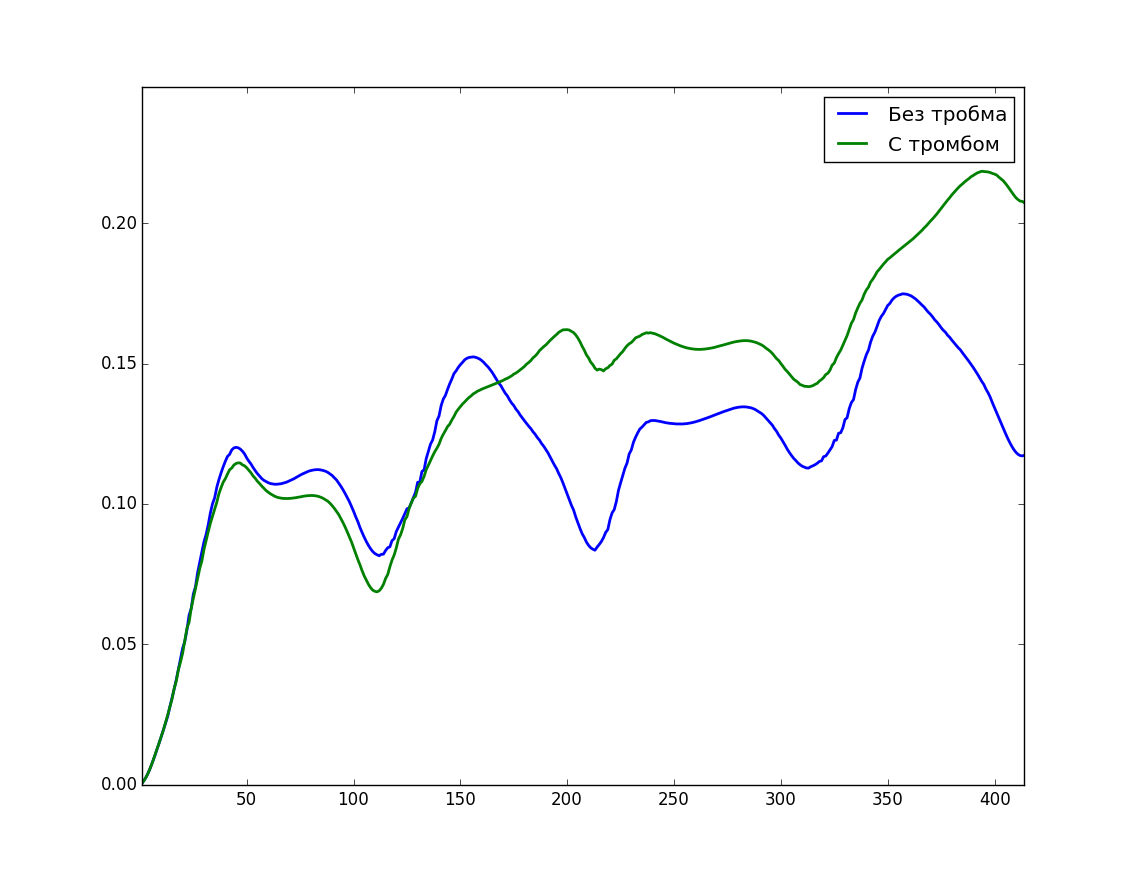
\includegraphics [scale=0.45] {forces_middle_point_thrombus.png}
  \caption{Сравнение напряжение в центре одной створки для случаев
           с наличием сгустка примеси, проходящего сквозь клапан,
           и без него.}
\label{img:forces_thrombus_comparison}
\end{figure}

Т.к. в данной работе мы рассматриваем два вида клапанов, естесственным является
желание их сравнить, чтобы понять, какие именно изменения вносят реалистичная
геометрия искусственного клапана по отношению к его <<идеальной>> версии. Одним
из параметров, по которым мы можем провести сравнение - это
итоговое распределение напряжения $F(q, r, s, t)$ по поверхности клапана в разные моменты времени.
Для клапана <<Юнилайн>> результирующее распределение показано на рис. \ref{img:uniline_stress_distribution}).
Параметры расчета идентичны \ref{img:uniline_dynamics}.

\begin{figure}[H]
  \center

  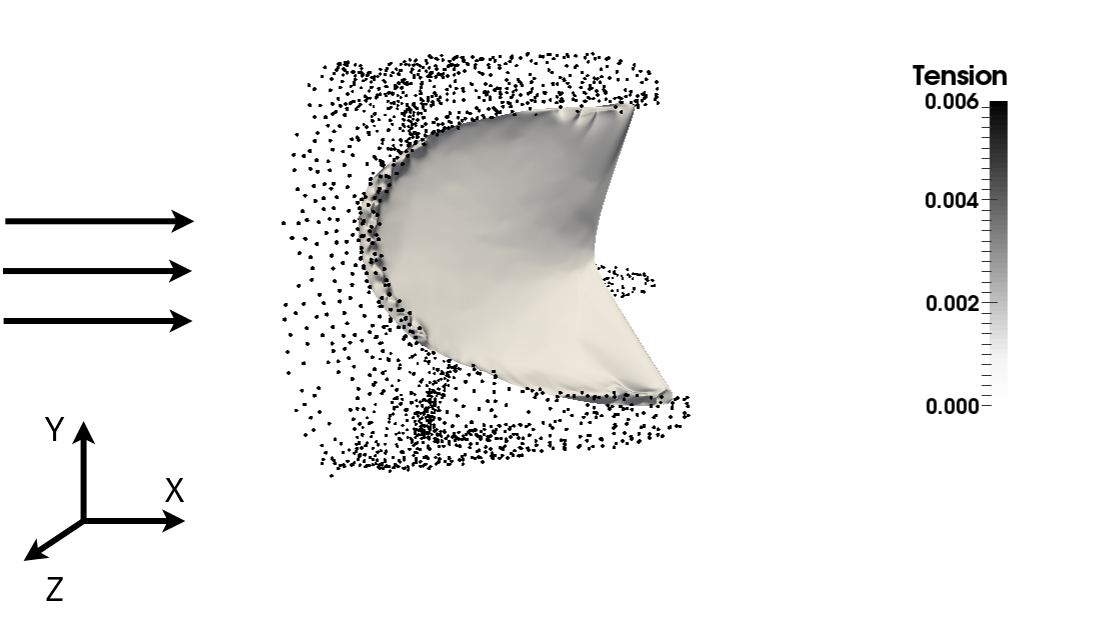
\includegraphics [scale=0.27] {uniline_stress_1_better_axes.png}

  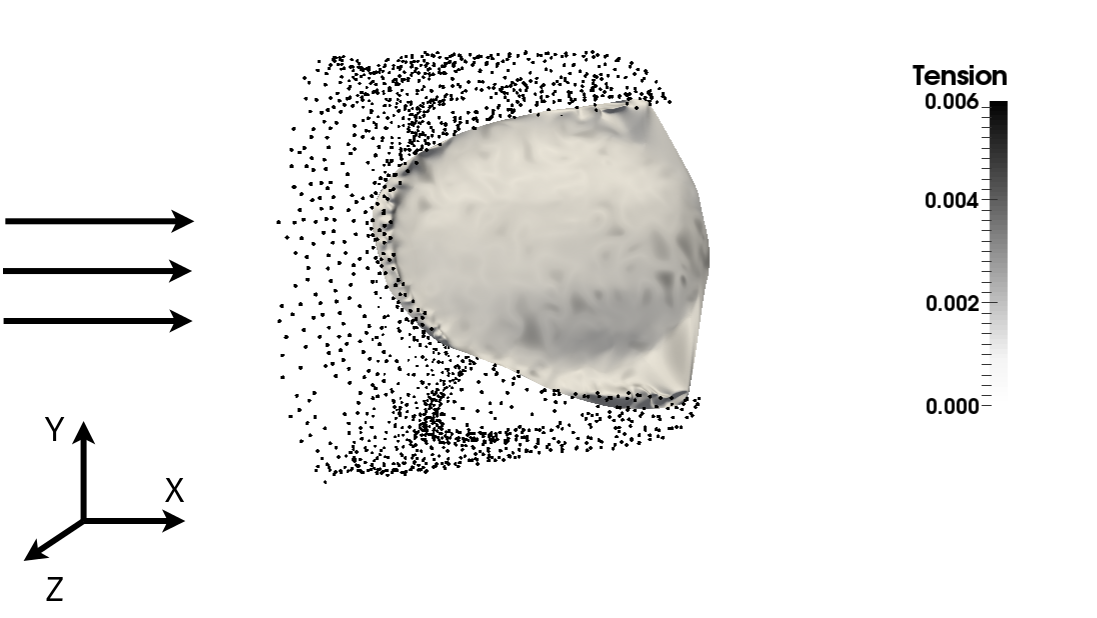
\includegraphics [scale=0.27] {uniline_stress_2_better_axes.png}

  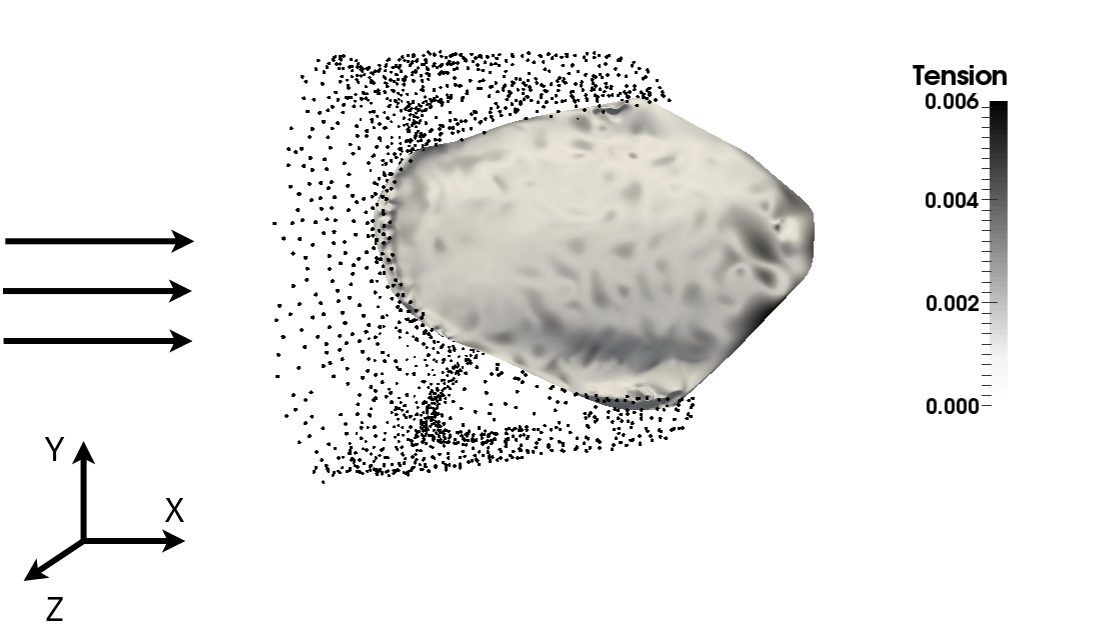
\includegraphics [scale=0.27] {uniline_stress_3_better_axes.png}

  \caption{Распределение напряжение по поверхности одной створки в моменты времени $t=0,
    t=0.4, t=0.8$. Точками обозначена поверхность фиброзного кольца}

\label{img:uniline_stress_distribution}
\end{figure}

Как видно из сравнения рис. \ref{img:valve_stress_distribution} и рис. \ref{img:uniline_stress_distribution},
в отличии от клапана идеальной формы, в момент наибольшего раскрытия в области
крепления створки <<Юнилайн>> не происходит значительного увеличения
поверхностного напряжения.

Одним из интересных эффектов, обнаруженных при моделировании, является эффект закручивания лепестков
клапана в некоторых случаях при его закрытии. Для возникновения такого эффекта необходимо рассматривать
такую геометрию клапана, которая в закрытом состоянии приводит к исбытку материала, т.е. сосуд может
быть закрыт лепестками меньшего размера. Этот эффект также описан в работе \cite{stapleton2015effect},
и наблюдался в лабораторных условиях. Результат моделирования работы клапана с появлением закручивания
можно увидеть на рис. \ref{img:valve_rotation}. Клапан симметричной формы в
начальный момент времени закрыт. Для створок клапана заданы коэффициенты
сопротивления растяжению $k_s = 8 \cdot 10^{3}$ и скручиванию $k_b = 2 \cdot 10^{3}$.
Внутри сосуда течет вязкая однородная несжимаемая жидкость $\rho=1$,
$\mu=1\cdot10^{-2}$, $p_{int}=0$, $p_{out}=6$. Давление жидкости на уже закрытый
клапан приводит к тому, что в силу переизбытка материала створок возникает
закручивание по часовой стрелке.

\begin{figure}[H]
  \center

  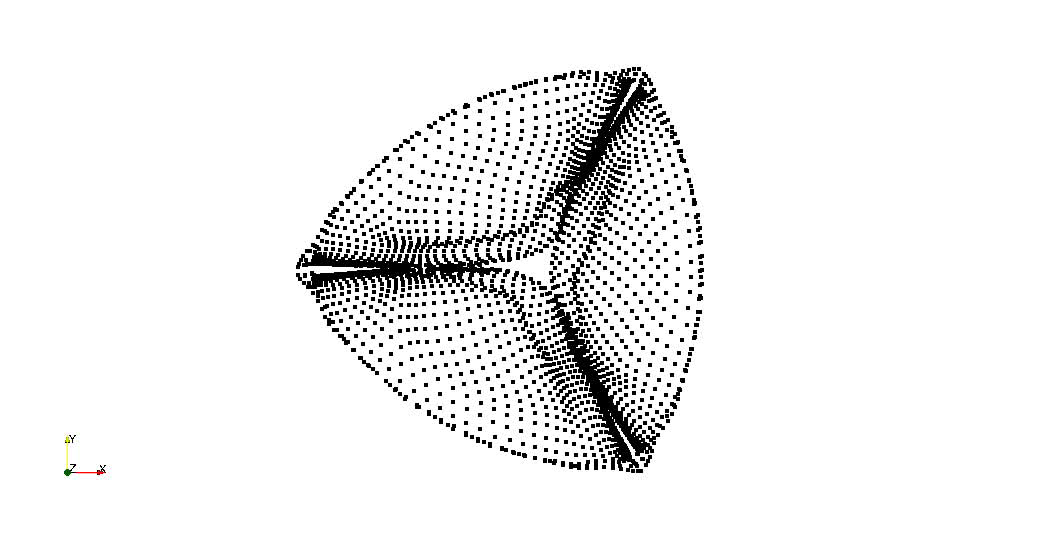
\includegraphics [scale=0.27] {rotation_1.png}

  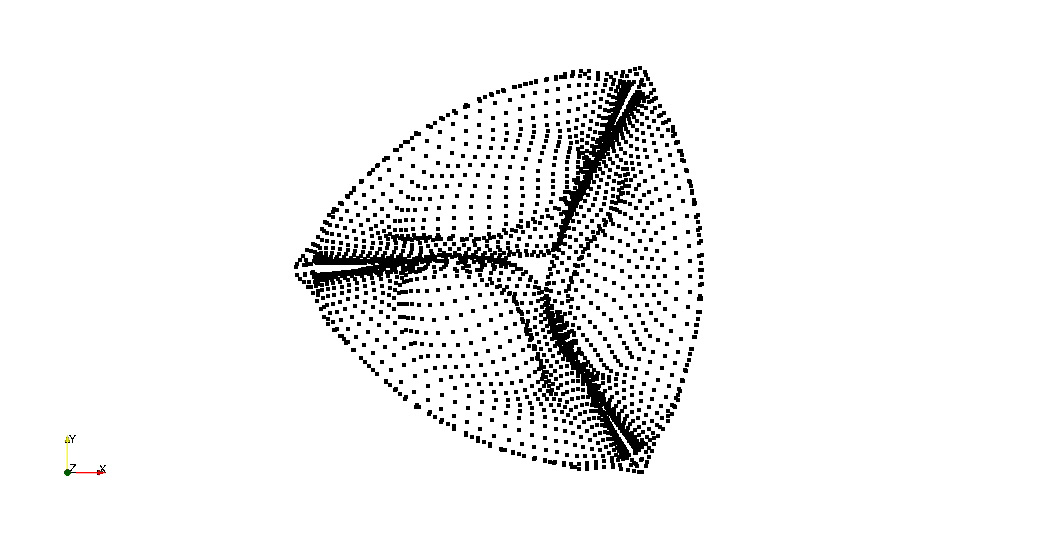
\includegraphics [scale=0.27] {rotation_2.png}

  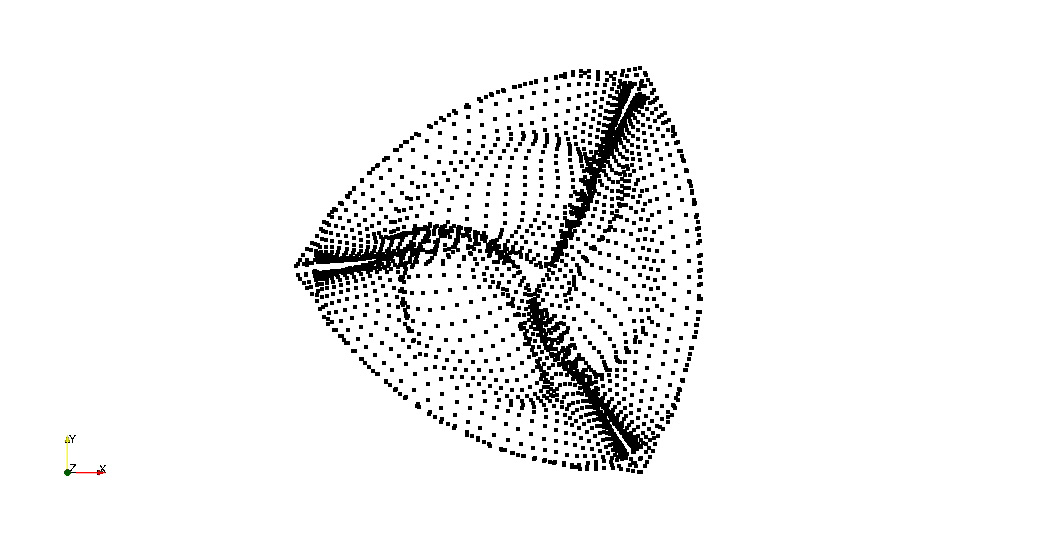
\includegraphics [scale=0.27] {rotation_3.png}

  \caption{Эффект <<закручивания>> лепестков клапана. Точками обозначены
      створки клапана в моменты времени $t=0, t=0.3, t=0.6$}

\label{img:valve_rotation}
\end{figure}

\section{Верификация модели} \label{sect3_3}

Для того, чтобы провести верификацию модели, описанной в \ref{chapt1}, было выбрано два подхода:

\begin{itemize}
    \item Сравнение результатов моделирования с лабораторными экспериментами на базе ФГБУ НИИ КПССЗ СО РАМН, г. Кемерово
    \item Сравнение результатов моделирования с работами других авторов
\end{itemize}

В качестве стенда для лабораторного эксперимента использовался аппарат Pulse Duplicator System от Vivitro labs,
изображение которого приведено на рис. \ref{img:pulse_duplicator_system}.

\begin{figure}[H]
  \center
  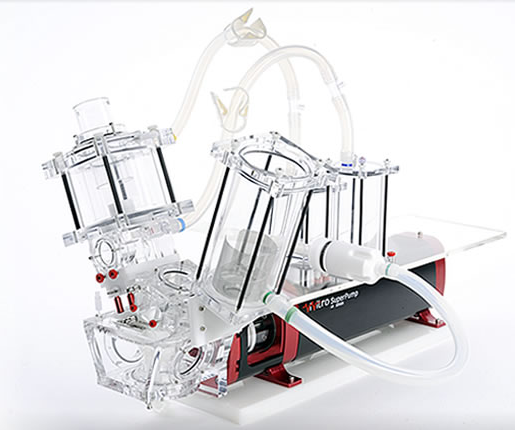
\includegraphics [scale=0.45] {pulse_duplicator_system.png}
  \caption{Pulse Duplicator System от Vivitro labs}
\label{img:forces_thrombus_comparison}
\end{figure}

Установка позволяет задавать различные формы давление (аорта, предсердие). В
качестве жидкости используется салин (0.9\% раствок NaCL). Установка позволяет
генерировать поток в диапазоне 2 - 15 л/мин, и частоту сердцебиения 30 - 220
ударов в минутую В нормальных условиях аортальное давление варьируется от 80 до
120 мм рт. ст. В качестве выходных данных может быть получены значения
пристеночного давления рядом с клапанами, расход жидкости, а также проведено
прямое наблюдение за работой стенда.

Для сравнения с данной установкой было проведено моделирование работы клапана
<<Юнилайн>> в размерных переменных на протяжении $0.8$с.
Для моделирования использовалось физиологическое давление (см. рис. \ref{img:physiological_pressure}),
где для $p_{in}$ бралось значение давления в предсердии $LA$, а для $p_{out}$ - давление в желудочке $LV$,
коэффициенты сопротивления растяжению $k_s = 5 \cdot 10^{2}$ и скручиванию
$k_b = 1 \cdot 10^{2}$.
Внутри сосуда течет вязкая однородная несжимаемая жидкость $\rho=1 \cdot 10^3 kg \cdot m^{-3}$, $\mu=0.25\cdot10^{-3} Pa \cdot s$.
Для расчета задавалась конечно-разностная сетка $\tilde{\Omega_h}$, соответствующая области течения,
и неструктурированная сетка $\tilde{\Gamma_h}$, соответствующая стенками сосуда и створкам клапана.
Расстояние между узлами $\tilde{\Omega_h}$ $h_x = h_y = h_z = 0.002 m$.
Для рассчета был выбран шаг по времени $\triangle t = 1 \cdot 10^{-4}$.
Длинна сосуда $l=0.1 m$, радиус $r=0.03 m$

\begin{figure}[H]
  \center
  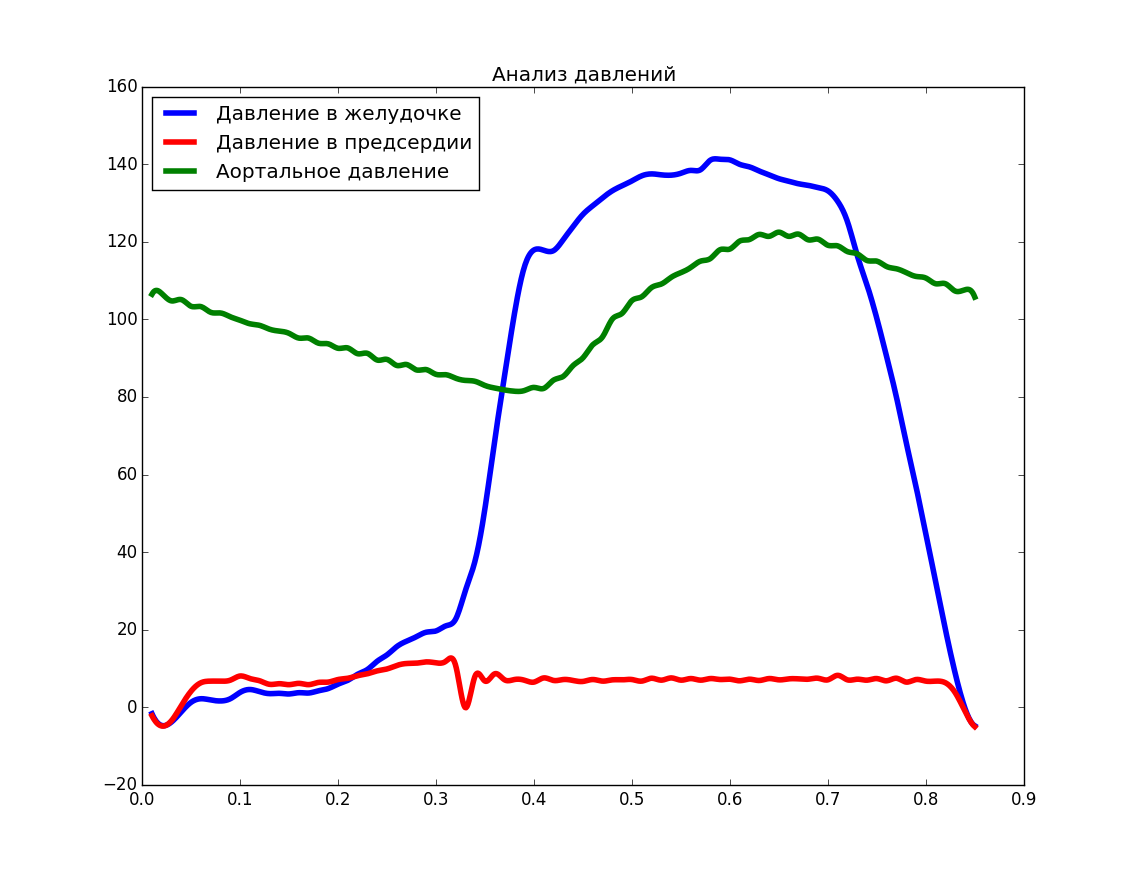
\includegraphics [scale=0.45] {physiological_pressure.png}
  \caption{Физиологическое давление}
  \label{img:physiological_pressure}
\end{figure}

На рис. \ref{img:pulse_duplicator_comparison} представлено сравнение расхода
жидкости, полученной для экспериментальной установки, с результатами моделирования.
График расхода жидкости, полученный в результате моделирования, хорошо совпадает
с экспериментальными даннымы на этапе раскрытия и закрытия клапана, но отличается
на этапе прохождения жидкости сквозь него.

\begin{figure}[H]
  \center
  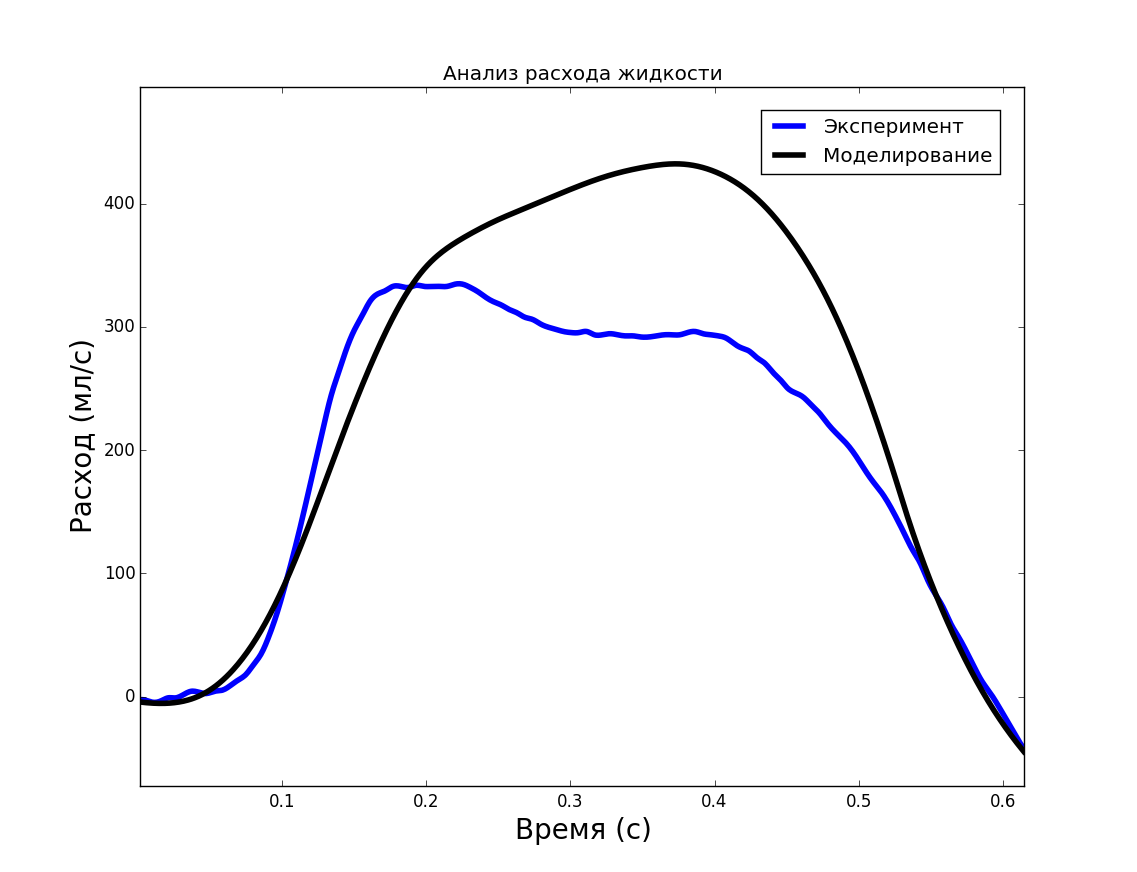
\includegraphics [scale=0.45] {pulse_duplicator_comparison.png}
  \caption{Сравнение расхода жидкости для эксперимента}
  \label{img:pulse_duplicator_comparison}
\end{figure}

Для сравнения со сторонними источниками была выбрана работа \cite{griffith2012immersed}. В ней
представлены результаты моделирования аортального клапана также при физиологическом давлении,
где $p_{in}$ - значение давления в желудочке $LV$, а для $p_{out}$ - давление в аорте $AO$.
В указанной работе было несколько отличий от данного исследования в постановке задачи.
Во первых, в форме сосуда были учтены синусы Вальсальвы, в то время как сосуд в нашей
постановке задачи имеет ровные стенки. Во-вторых, в нашей работе учтено наличие фиброзного
кольца, тогда как в исследовании \cite{griffith2012immersed} створки крепятся напрямую к стенкам сосуда.

На рис. \ref{img:griffith_comparison} приведены графики расхода жидкости, полученные при моделировании
в данной работе, и их сравнение с исследованием \cite{griffith2012immersed}. Они показывают достаточно
хорошее совпадение почти по всем параметрам, несмотря на указанные выше отличия.

\begin{figure}[H]
  \center
  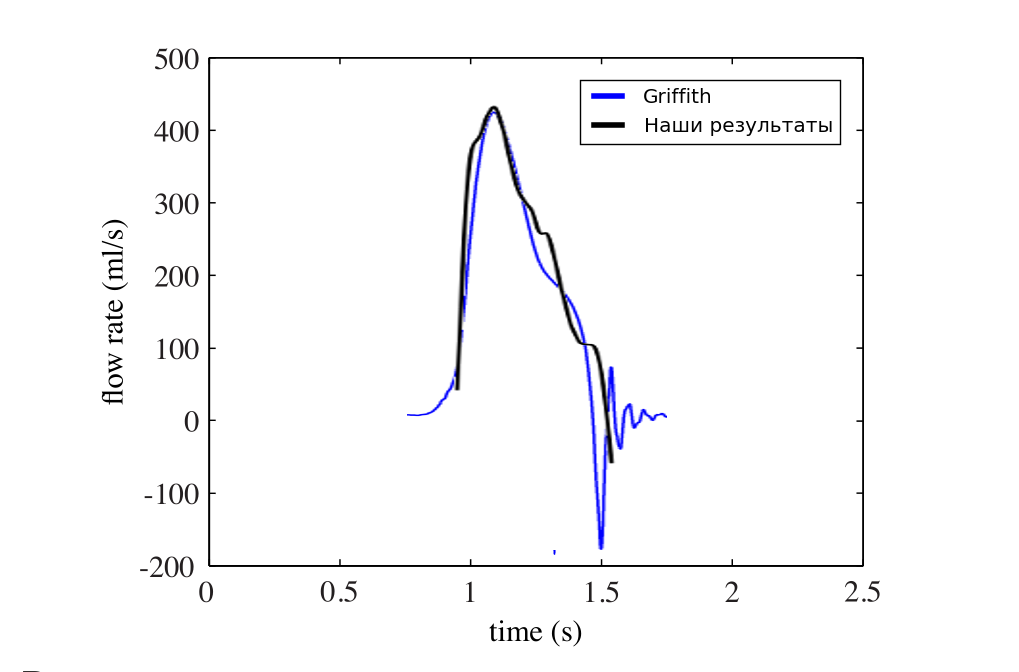
\includegraphics [scale=0.45] {griffith_comparison.png}
  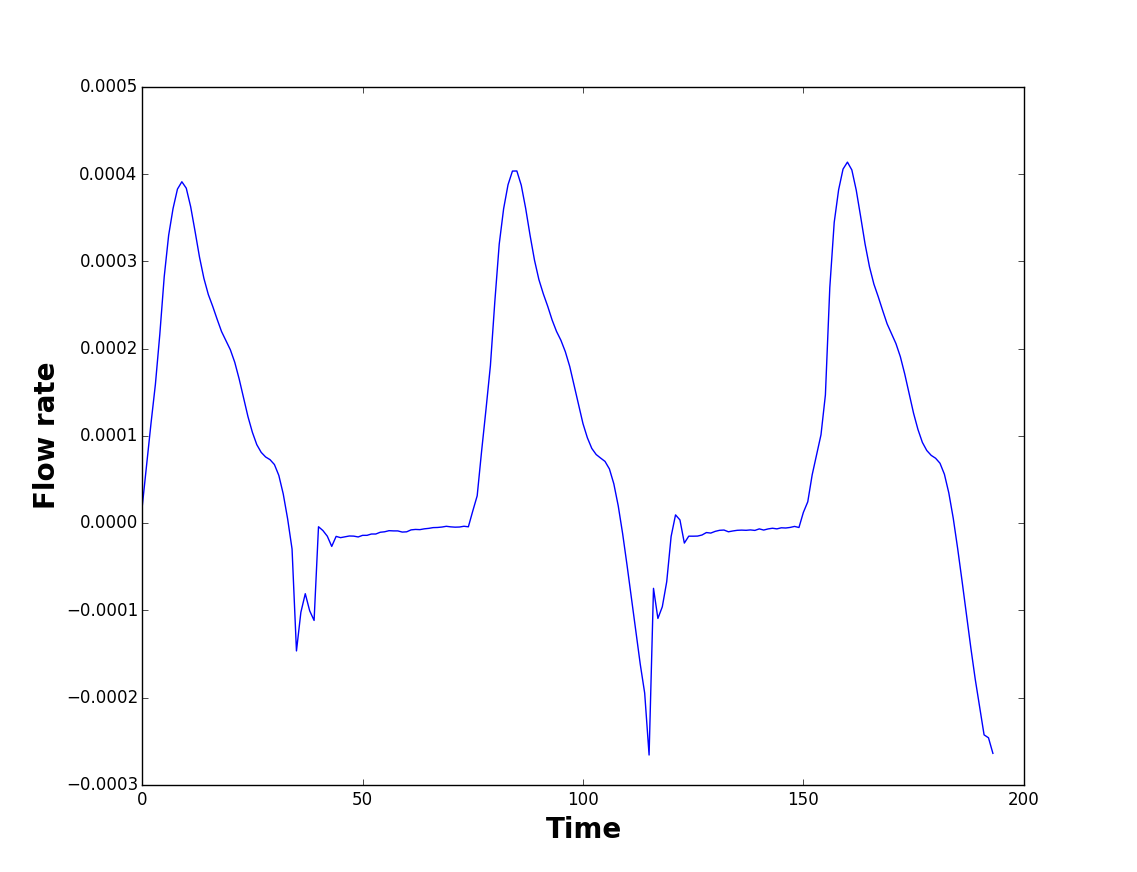
\includegraphics [scale=0.45] {flow_rate_aorta.png}
  \caption{Сравнение расхода жидкости для других авторов}
  \label{img:griffith_comparison}
\end{figure}

\clearpage
